\subsection{Descri\c c\~ao das Etapas}

\textbf{An\'alise explorat\'oria dos dados (EDA)}
a partir da \ref{etp:1}, foi realizado o EDA (do inglês \textit{Exploratory Data Analysis}) para processar os dados obtidos até o momento. A análise exploratória de dados foi promovida por John Tukey \cite{Bandara2021} como uma abordagem para explorar os dados, resumir suas principais características e formular hipóteses que possam direcionar a coleta adicional de dados e experimentos. No contexto de análises de dados, várias técnicas de EDA têm sido adotadas.
Nessa análise da EDA, serão abordadas várias análises, como a correlação de Pearson, para iniciar e verificar quais variáveis podem ser excluídas como ruído e não têm correlação com a variável LT01. Nesse caso, as variáveis retiradas são consideradas negativas e têm pouca correlação com o LT01, as únicas variáveis que apresentam correlação negativa são B3 e FT02, mesmo sendo uma correlação negativa, essas variáveis possuem uma correlação inviável ou próxima de $0$, levando à decisão de removê-las.

Uma análise bem feita do EDA mostra tudo que os dados podem ter. Esses dados fornecidos pela companhia SANEPAR são coletados em campo por hora, como por exemplo, a cada hora possui um valor esperado. Nisso, pode haver os famosos NaN, que representam a falta de dado coletado, como em um dia em que as bombas podem ter ido para manutenção. Esses NaNs também podem ser registrados como uma anomalia nos dados.

A Figura \ref{fig:person} mostra a correlação entre as variáveis no conjunto de dados em questão. Essa imagem representa graficamente a relação entre as variáveis e é usada para evidenciar a existência de uma correlação forte no valor de $0,97$ é considerada forte entre elas, quanto mais próximo do valor $1$ a correlação é sempre forte e $0,9$ para mais ou para menos indica uma correlação muito forte, 0 a $0,3$ positivo ou negativo indica uma correlação desprezível.

\begin{figure}[!htb]
	\centering
	\caption{Correlação de Pearson}
	\label{fig:person}
	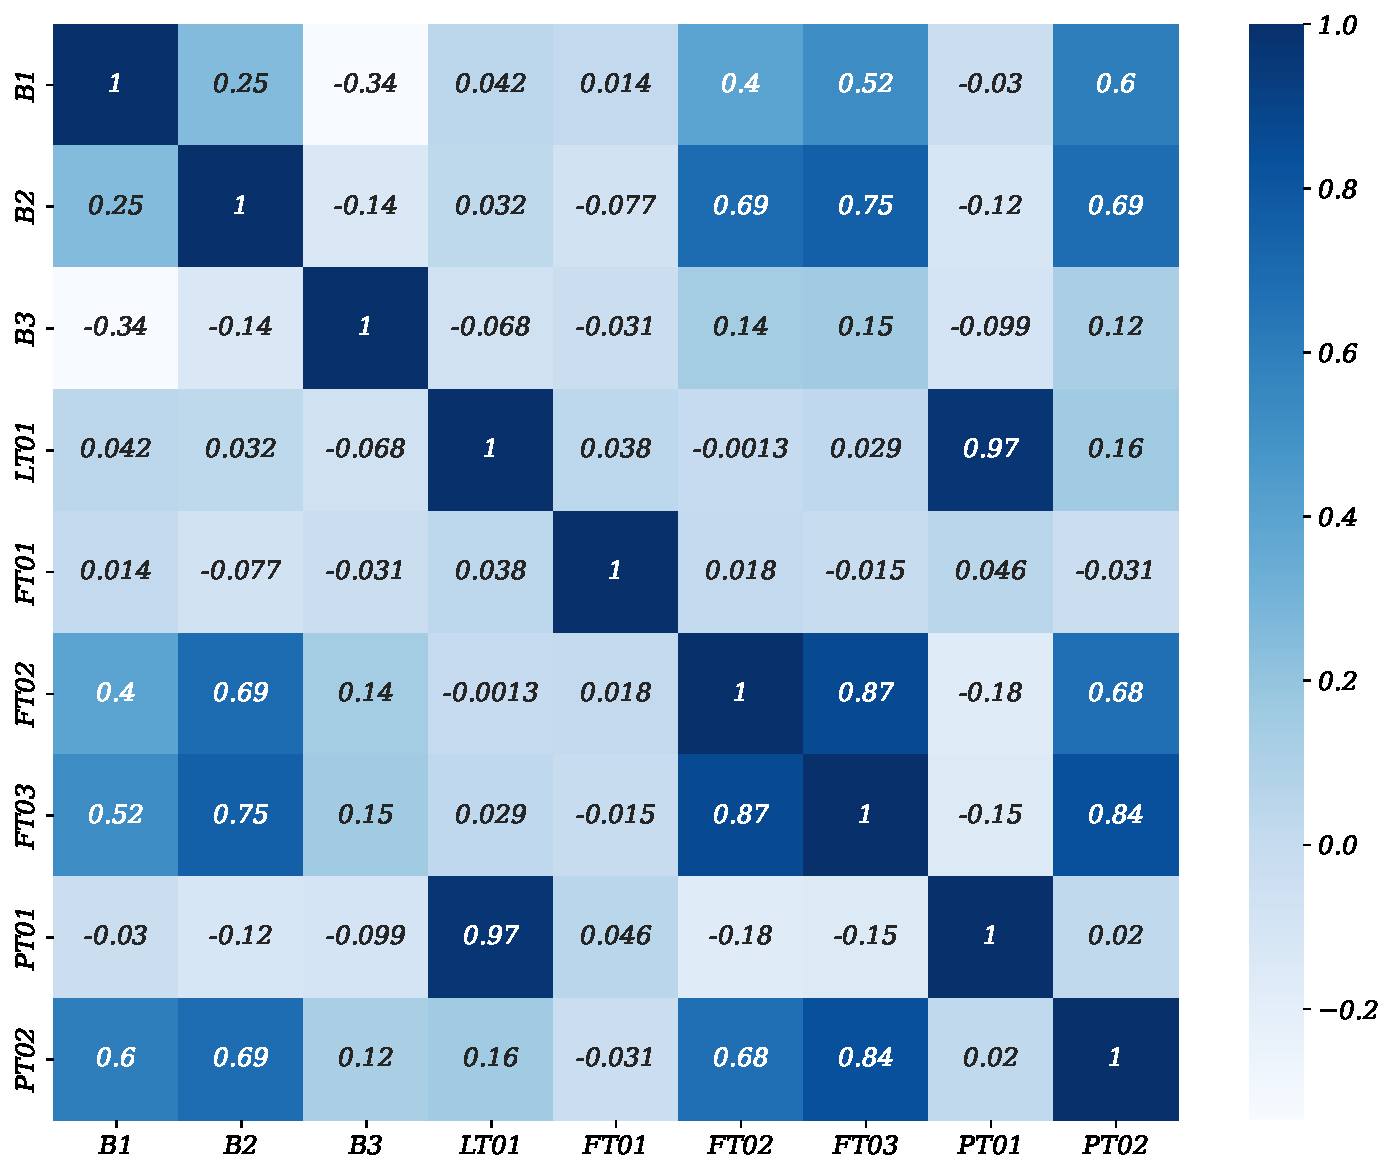
\includegraphics[width=0.7\linewidth]{Resultados/Figuras/person}
	
	
\end{figure}

Nesse conjunto de dados que está sendo trabalhado, há uma forte correlação da variável PT01 nos modelos de LR e DTR (do inglês \textit{Decision Tree Regressor}). Esses modelos foram escolhidos para trabalhar com o LT01 como entrada e o PT01 como saída. A Figura \ref{fig:lr-lt01-m3} fornece uma representação dos coeficientes $\beta_0$ e $\beta_1$. Um aumento de $1$ na variável $x$ está associado a um aumento proporcional de $\beta_1$ na variável $y$. O valor de $\beta_0$ representa o valor de $y$ quando $x$ é igual a $0$.

\begin{figure}[!htb]
	\centering
	\caption{Regressão linear LT01 vs PT01 correlação 97\%}
	\label{fig:lr-lt01-m3}
	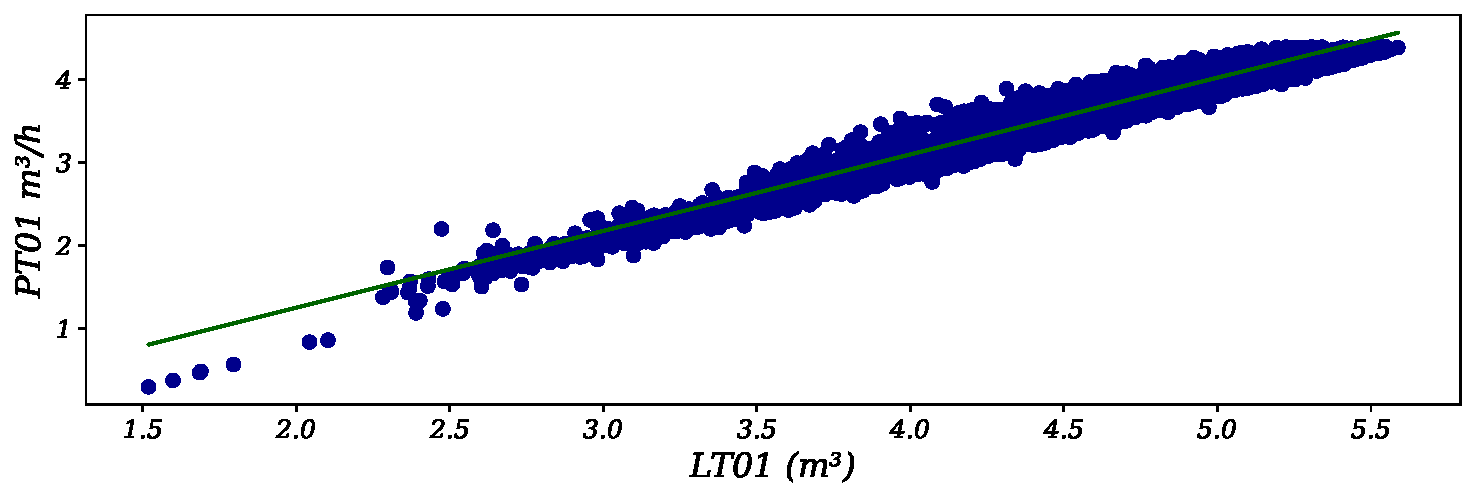
\includegraphics[width=0.7\linewidth]{Resultados/Figuras/LR}
	
	
\end{figure}








A Tabela \ref{tb:est}, o desvio padrão é representado pela sigla STD, que corresponde à expressão em inglês \textit{standard deviation}. Assim como em qualquer empresa de tratamento de água, é utilizado um mecanismo de acionamento automático denominado ``trava de segurança'' para evitar que o nível do tanque se aproxime de zero e haja falta de água nos locais abastecidos por esse tanque. O nível máximo que o tanque pode alcançar é de $5,26 m^3$ (equivalente a $5264.56$ litros). As bombas são ativadas em sua potência máxima para evitar que sejam acionadas quando o nível do tanque estiver dentro dessa faixa. No entanto, a bomba $1$ ainda estaria operando para completar o nível do tanque caso esteja dentro dessa faixa. Nessa Tabela \ref{tb:est}, foram filtrados os horários de pico nos quais pode ocorrer a maior demanda d'água.

\begin{table}[!htb]
	\centering
	\caption{Descrição estatística dos dados com o filtro aplicado das 18h às 21h}\label{tb:est}
	\begin{tabular}{@{}cccccccccc@{}}
		\toprule
		\multicolumn{1}{l}{\textbf{18h a 21h}} & \multicolumn{1}{c}{\textbf{B1}} & \multicolumn{1}{c}{\textbf{B2}} & \multicolumn{1}{c}{\textbf{B3}} & \multicolumn{1}{c}{\textbf{LT01}} & \multicolumn{1}{c}{\textbf{FT01}} & \multicolumn{1}{c}{\textbf{FT02}} & \multicolumn{1}{c}{\textbf{FT03}} & \multicolumn{1}{c}{\textbf{PT01}} & \multicolumn{1}{c}{\textbf{PT02}} \\ \midrule
		\textbf{Contagem}                      & 2921                            & 2921                            & 2921                            & 2921                              & 2921                              & 2921                              & 2921                              & 2921                              & 2921                              \\
		\textbf{Média}                         & 55,98                           & 30,60                           & 5,26                            & 3,18                              & 86,52                             & 132,87                            & 117,62                            & 4,04                              & 22,55                             \\
		\textbf{STD}                           & 10,00                           & 15,63                           & 15,57                           & 0,67                              & 124,41                            & 18,48                             & 12,83                             & 0,71                              & 2,92                              \\
		\textbf{Min.}                          & 0                               & 0                               & 0                               & 0,29                              & 0                                 & 0                                 & 0,03                              & 0,88                              & 0                                 \\
		\textbf{25\%}                          & 57,99                           & 31,63                           & 0                               & 2,77                              & 0                                 & 123,40                            & 112,52                            & 3,61                              & 21,98                             \\
		\textbf{50\%}                          & 57,99                           & 35,20                           & 0                               & 3,24                              & 0,12                              & 132,88                            & 118,18                            & 4,10                              & 22,87                             \\
		\textbf{75\%}                          & 57,99                           & 38,17                           & 0                               & 3,71                              & 258,48                            & 142,89                            & 124,48                            & 4,59                              & 23,05                             \\
		\textbf{Max.}                          & 59,99                           & 59,99                           & 59,99                           & 4,39                              & 370,35                            & 277,94                            & 167,78                            & 5,31                              & 28,08                             \\ \bottomrule
	\end{tabular}
	
	
\end{table}



A realização da EDA consegue mostrar que os dados estão sendo coletados de maneira significativa, ao observar as correlações e possibilita trabalhar com as variáveis que apresentam correlação maior ou não negativa. Nos modelos ARIMA e seus antecessores, ele utiliza o ACF (do inglês \textit{\textit{Auto-Correlation Function}}) e o PACF (do inglês \textit{Partial Auto-correlation Function}) para analisar esses métodos. A análise destes métodos para o modelo ARIMA permite otimizar os parâmetros do modelo.

O ACF é uma medida estatística utilizada para identificar a presença de correlação serial em uma série temporal. Ele calcula a autocorrelação entre os valores da série em diferentes defasagens, ou seja, a correlação entre os valores atuais e os valores passados da série. 

O ACF é útil para analisar a dependência temporal dos dados e identificar padrões de sazonalidade, tendência ou outros efeitos temporais. Por meio do ACF, é possível avaliar se a série exibe autocorrelação significativa em defasagens específicas, o que pode indicar a presença de não estacionariedade ou estrutura temporal que precisa ser considerada na análise ou modelagem da série temporal.


A estatística ADF (do inglês \textit{Augmented Dickey-Fuller}) de $-12,515$ indica a evidência de estacionariedade na série temporal. Quanto mais negativo for o valor da estatística ADF, maior é a evidência de estacionariedade nos dados.

O valor de p, aproximadamente de $0,0000000000000000000000262$, expresso de forma mais concisa como $2,62\times 10^{-23}$ usando a notação científica, está associado ao teste ADF. Este valor-p representa a probabilidade de obter um resultado igual ou mais extremo do que o observado, sob a suposição de que a hipótese nula seja verdadeira. No contexto do teste ADF, a hipótese nula é a presença de raiz unitária na série temporal, indicando não estacionariedade. Portanto, um valor de p baixo, geralmente abaixo de um nível de significância predefinido, como $0,05$, sugere que a série temporal é estacionária, enquanto um valor de p alto sugere não estacionariedade. Dado o valor de p de $2,62\times 10^{-23}$, evidencia-se uma probabilidade muito baixa, indicando forte suporte contra a hipótese nula e sugerindo que a série temporal é estacionária. Na Tabela \ref{tb:adf}, são apresentados todos os dados do teste para estacionalidade.
Os resultados indicam fortes evidências contra a hipótese nula. Com um teste ADF de $-12,515 $ e um valor de p extremamente baixo de $2,62 \times 10^{-23}$, rejeita-se a hipótese nula de presença de raiz unitária. Os $44$ atrasos utilizados e as $17.477$ observações corroboram a análise estatística.

\begin{table}[!htb]
	\centering
	\caption{Teste de Dickey-Fuller Aumentado}\label{tb:adf}
	\begin{tabular}{lc}
		\hline
		Teste ADF & $-12,515$ \\ \hline
		Valor de p & $2,62 \times 10^{-23}$ \\
		Atrasos utilizados & $44$ \\
		Número de observações & $17.477$ \\
		Valor crítico $(1\%)$ & $-3,431$ \\
		Valor crítico $(5\%)$ & $-2,862$ \\
		Valor crítico $(10\%)$ & $-2,567$ \\
		\hline
	\end{tabular}
\end{table}




Ao comparar a estatística de teste ADF com os valores críticos, observa-se que está significativamente abaixo deles em todos os níveis de significância $(1\%, 5\%, 10\%)$. Portanto, a conclusão é de que os dados não possuem raiz unitária, indicando que são estacionários.

Na Figura \ref{fig:acfa}, pode-se observar a diferença entre a autocorrelação (ACF) exibida na Figura \ref{fig:acfa} e a autocorrelação parcial (PACF) exibida na Figura \ref{fig:pacf}. A autocorrelação é uma medida da correlação entre os valores da série temporal em diferentes defasagens, levando em consideração tanto a correlação direta quanto a correlação indireta. Por outro lado, a autocorrelação parcial mede apenas a correlação direta entre os valores, desconsiderando a influência das defasagens intermediárias. Essas análises são úteis para identificar padrões e relações de dependência entre os valores da série temporal, fornecendo informações importantes para a modelagem e previsão desses dados.
O intervalo de confiança padrão de 95\% é representado pela marca azul nas Figuras \ref{fig:acfa} e \ref{fig:pacf}. As observações que estão fora desse intervalo são consideradas estatisticamente correlacionadas, indicando a presença de padrões ou estrutura na série temporal.

A correlação visualizada na Figura \ref{fig:acfa} é fundamental para a interpretação do teste ADF. Em uma série de ruído branco, os valores são completamente aleatórios e não apresentam correlação significativa. Portanto, quando há correlação presente na série, isso indica a existência de padrões ou dependências entre os valores, o que pode ser explorado para a modelagem e previsão da série temporal.
\begin{figure}[!htb]
	\centering
	\caption{Autocorrelação}\label{fig:acfa}
	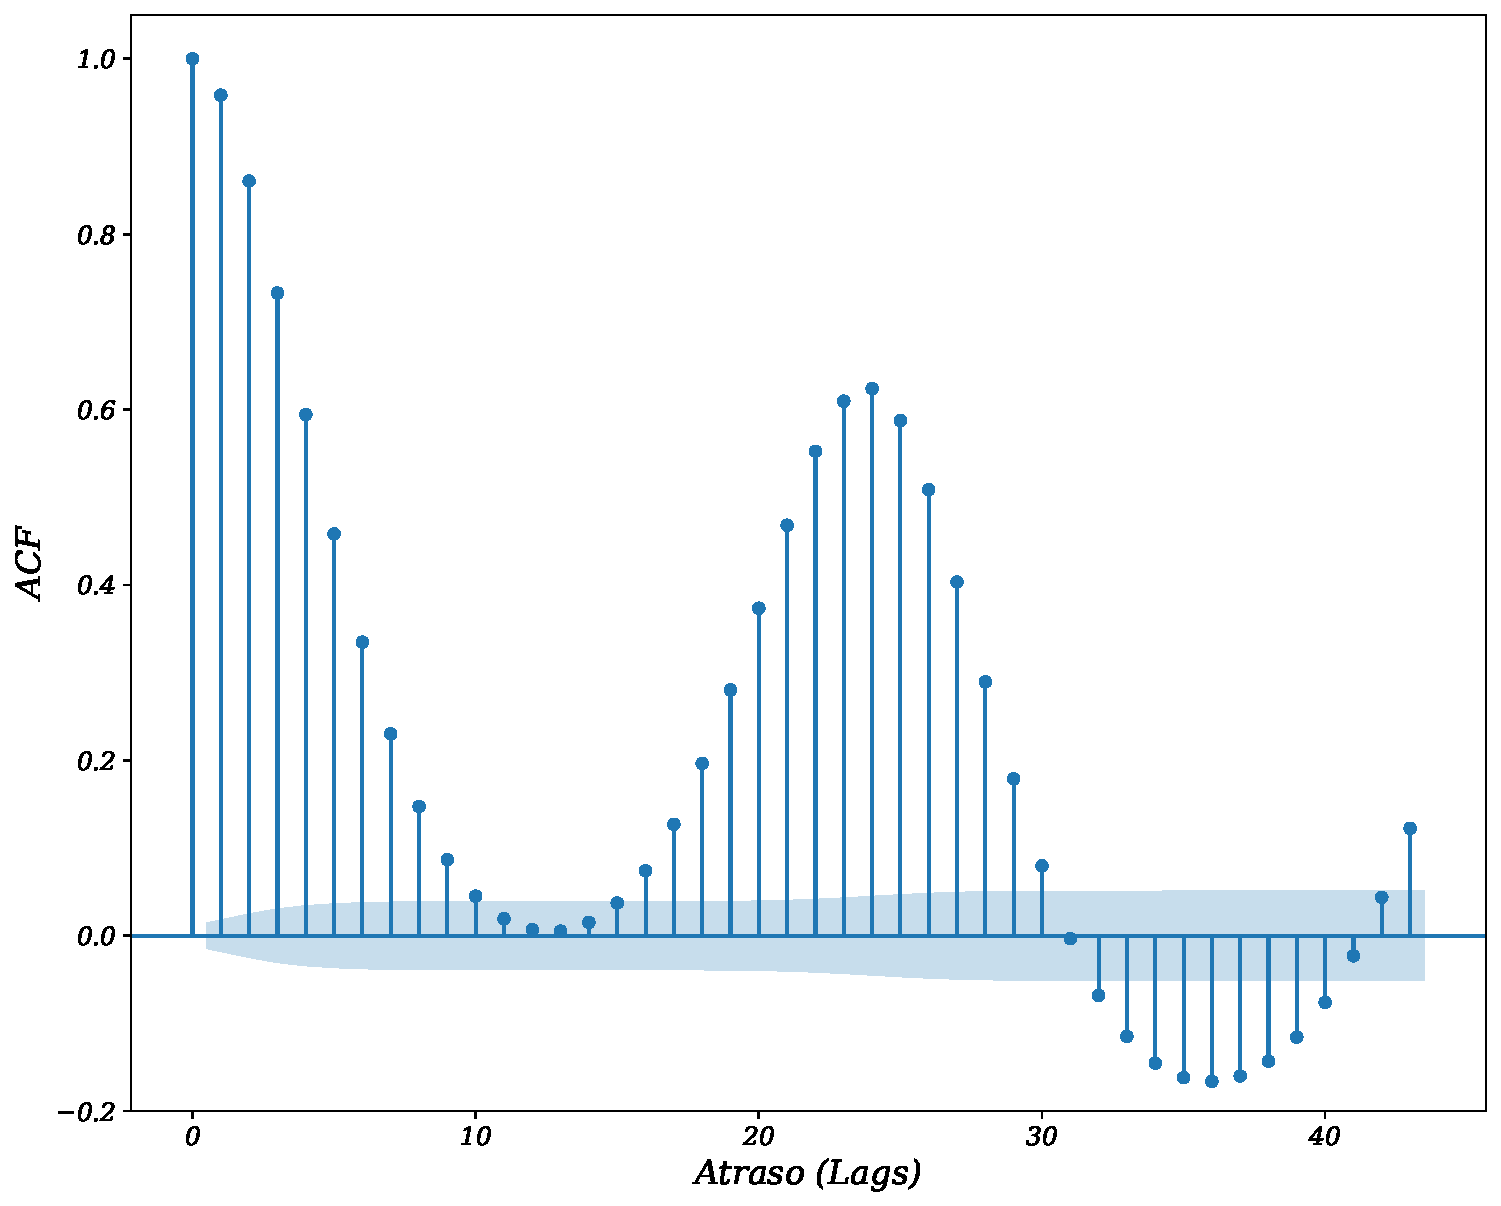
\includegraphics[width=0.7\linewidth]{Resultados/Figuras/acf} 
	
	
\end{figure}


\begin{figure}[!htb]
	\centering
	\caption{Autocorrelação parcial}\label{fig:pacf}
	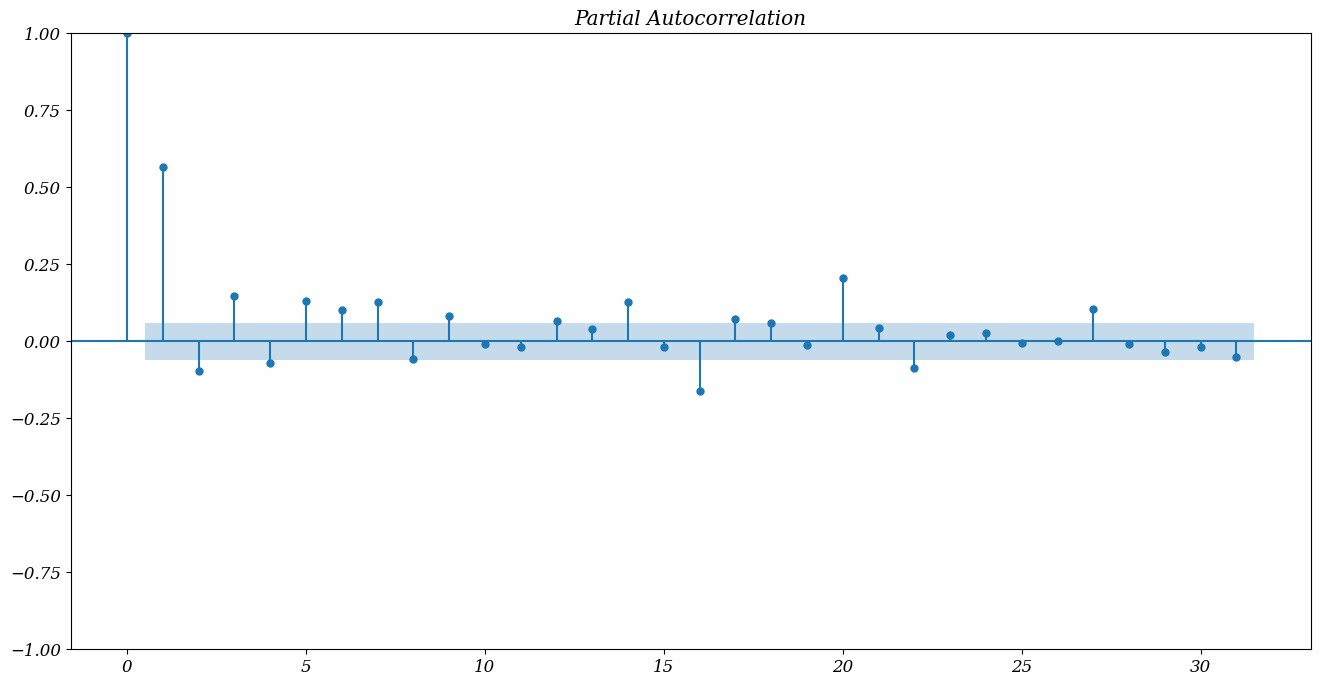
\includegraphics[width=0.7\linewidth]{Resultados/Figuras/pacf}
	
	
	
\end{figure}



Demonstrar que uma série temporal tem ou pode ter um ruído branco também é conveniente para a análise da EDA.
Na Figura \ref{fig:ruido-branco}, é possível observar uma série temporal que pode ser caracterizada como ruído branco. Uma série temporal é considerada ruído branco se suas variáveis forem independentes e distribuídas de forma idêntica, com média zero. Isso implica que todas as variáveis possuem a mesma variância ($\sigma^2$) e que cada valor não possui correlação com os demais valores da série.

\begin{figure}[!htb]
	\centering
	\caption{Ruído branco}
	\label{fig:ruido-branco}
	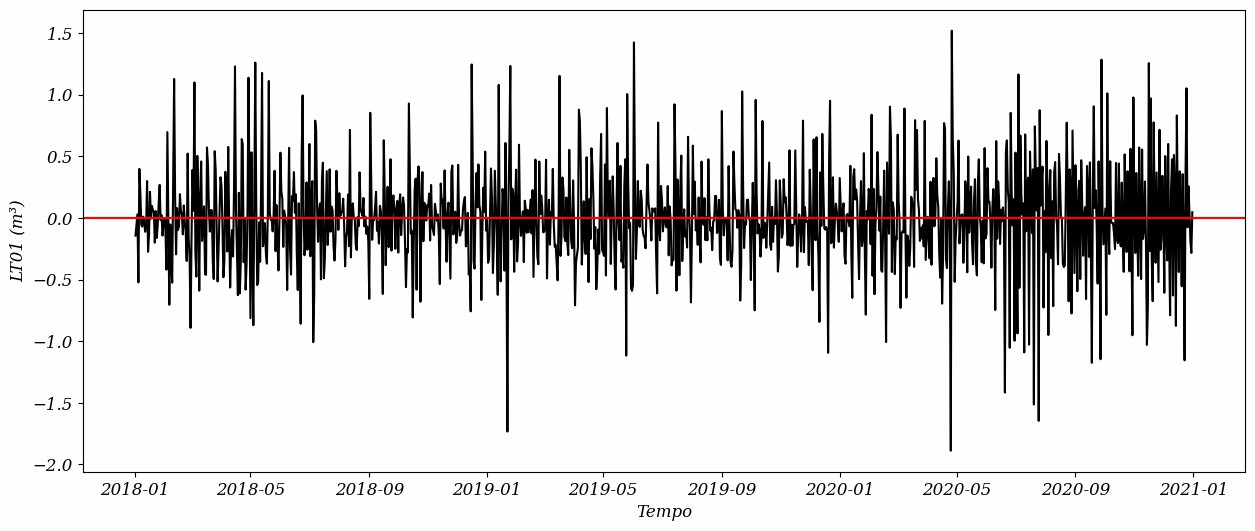
\includegraphics[width=\linewidth]{Resultados/Figuras/ruido-branco}
	
	
\end{figure}

Nesse exemplo, ao utilizar os dados da SANEPAR, a série temporal trabalhada é estacionária e também apresenta ruído branco (do inglês \textit{white noise}).



Com base na forte evidência contra a hipótese nula, podemos rejeitar a hipótese nula. A Figura \ref{fig:hist}, podemos notar um aumento na demanda durante essas horas durante o ano de 2019.
Conforme mencionado na subseção \ref{subsubsec:motivacao}, as anomalias climáticas ocorridas em 2020, especialmente a falta de chuvas e devido ao COVID-19, tiveram um impacto significativo nos resultados. Isso contribuiu para as mudanças observadas na demanda de água ao longo desse período.

\begin{figure}[!htb]
	\centering
	\caption{Violino no nível do reservatório}
	\label{fig:hist}
	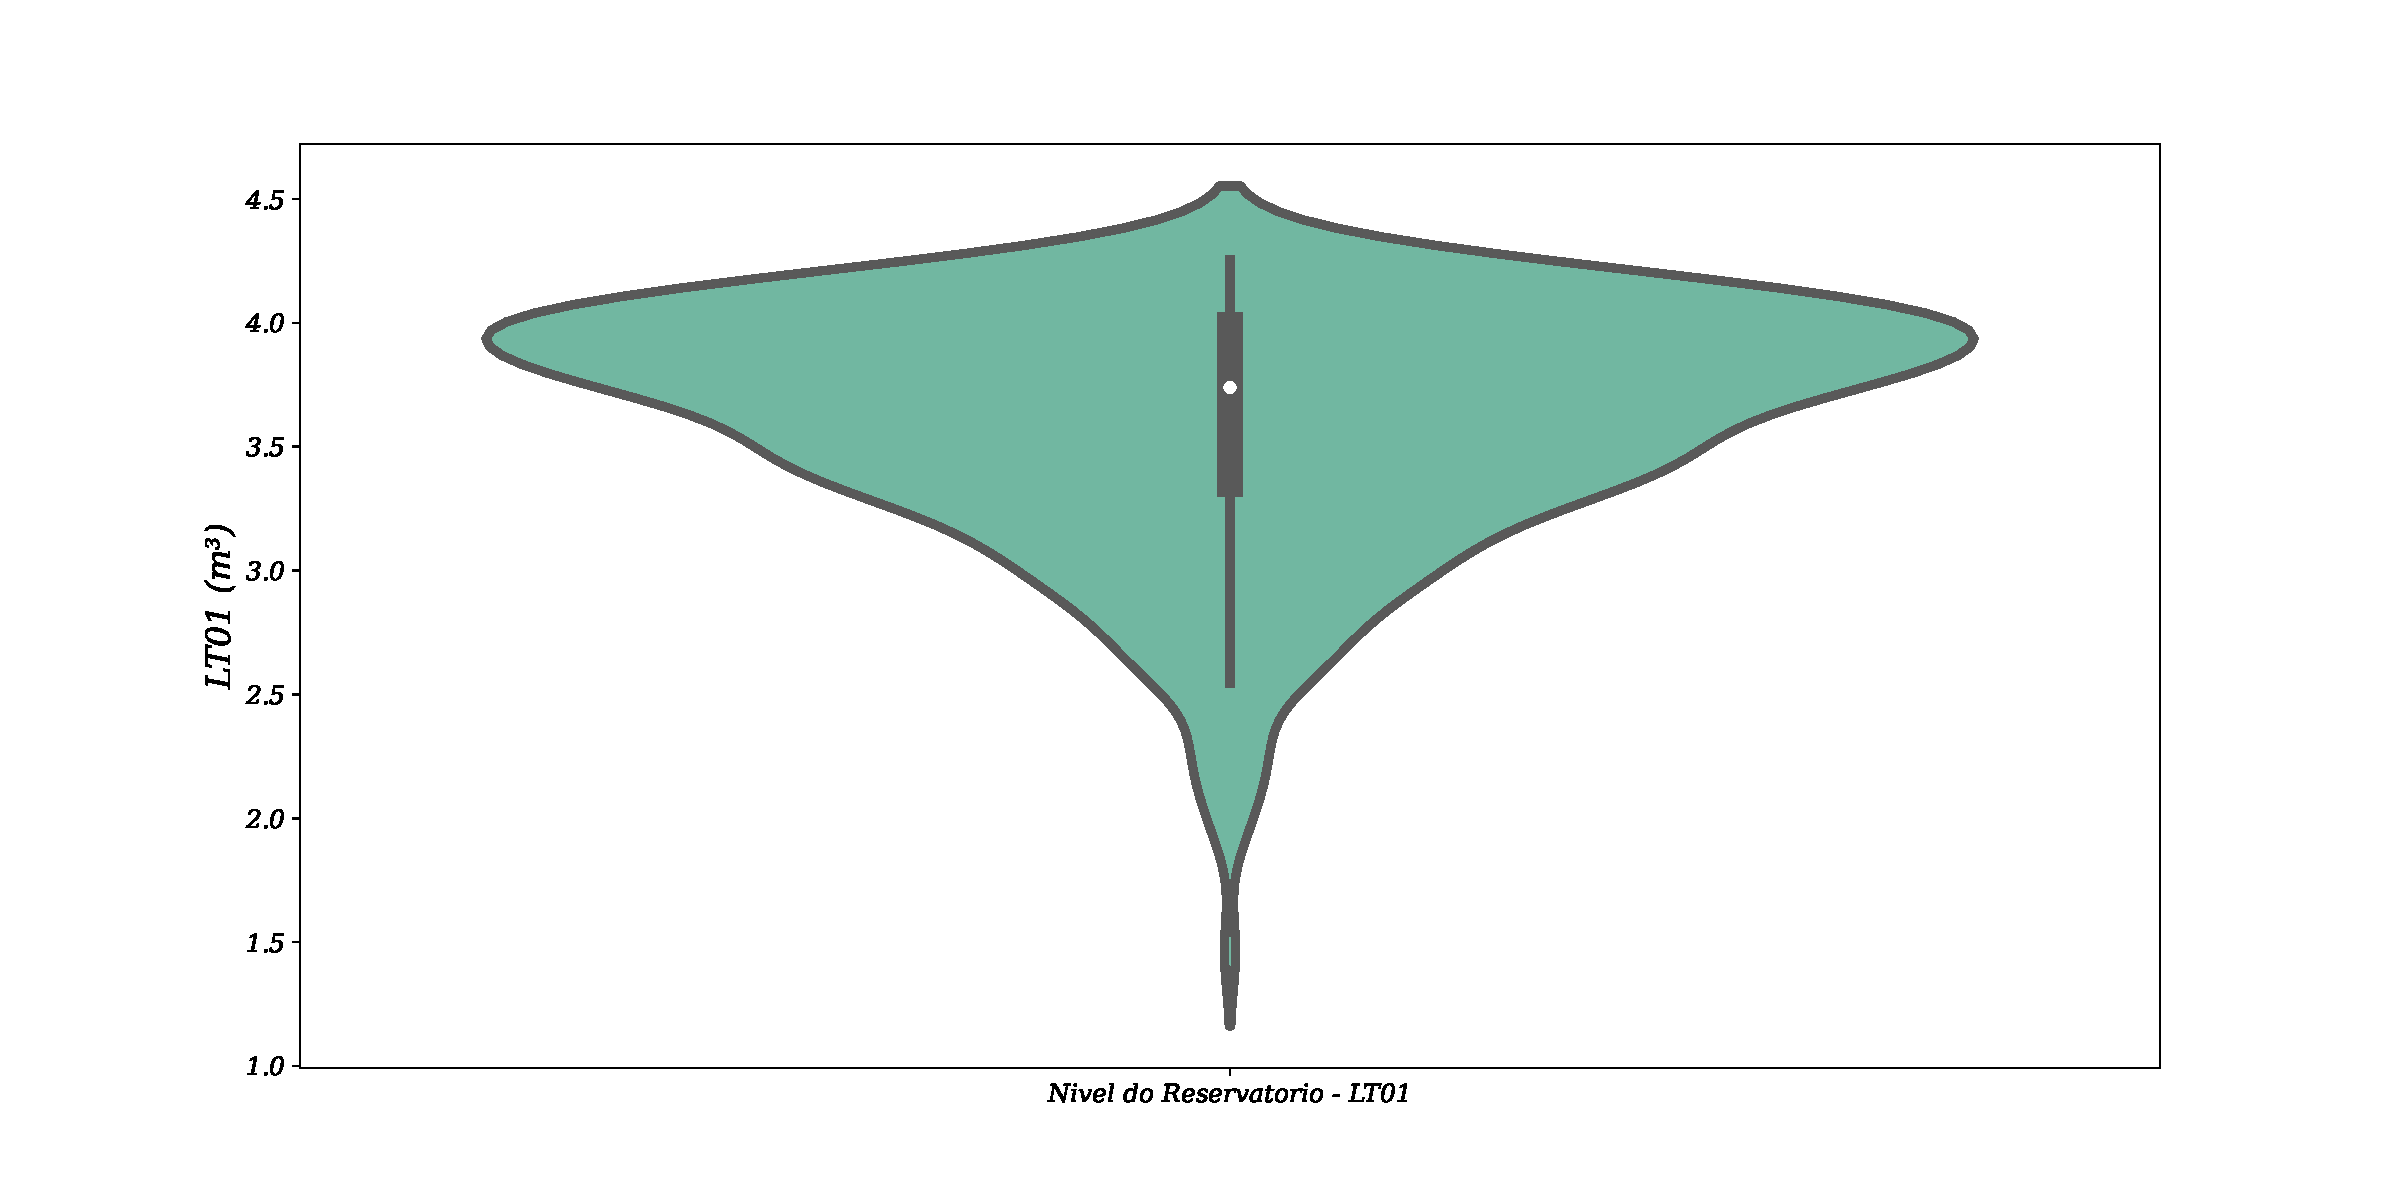
\includegraphics[width=0.7\linewidth]{Resultados/Figuras/viol}
	
	
\end{figure}





A Figura \ref{fig:ft03} mostra como a vazão pode ser afetada pelo nível do tanque. É interessante observar que a vazão de recalque tem um impacto mais significativo no nível do tanque em comparação com as outras vazões. Isso ocorre porque a vazão de recalque está associada à injeção de água diretamente no tanque por meio da bomba localizada próxima à base do tanque. Por outro lado, as demais vazões apresentam alguns valores ausentes, o que limita sua influência na análise geral.	


\begin{figure}[!htb]
	\centering
	\caption{Violino da vazão de recalque}
	\label{fig:ft03}
	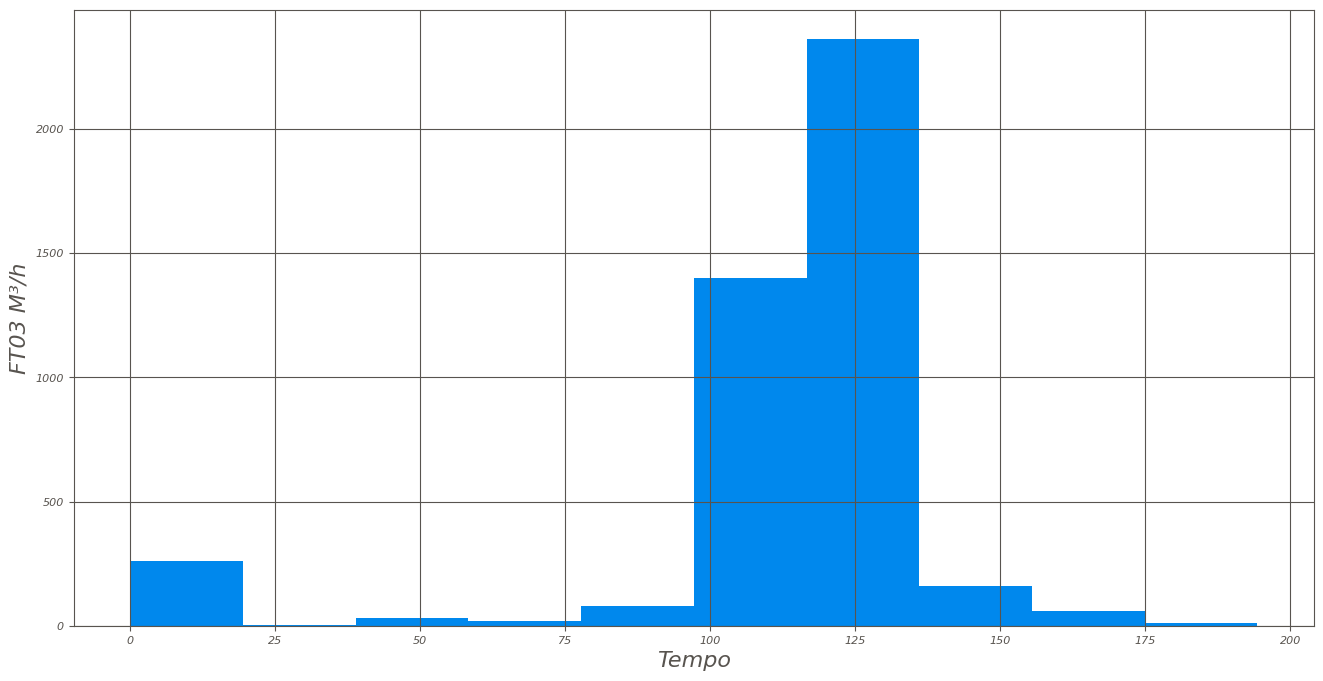
\includegraphics[width=0.7\linewidth]{Resultados/Figuras/ft03}
	
	
\end{figure}




\textbf{M\'ultiplas entradas e sa\'ida \'unica (MISO)}
na etapa \ref{etp:2}, foi explorado o modelo MISO (do inglês \textit{Multiple Inputs, Single Output}) na dissertação. O modelo ARIMA, juntamente com suas variantes e extensões, foi amplamente estudado durante a pesquisa, assim como modelos regressivos que envolvem múltiplas variáveis de entrada e uma variável de saída, neste caso, a LT01. As demais variáveis foram utilizadas como suporte para melhorar o modelo do tipo ARIMAX ou modelos com variáveis exógenas. Quando aplicado sem o uso de variáveis exógenas, o modelo ARIMA apresenta apenas uma entrada, semelhante ao modelo de LR. No entanto, ao incluir variáveis exógenas, o modelo se torna MISO, permitindo uma modelagem  abrangente e considerando a interação de várias variáveis para prever a variável de interesse.


\textbf{Decomposi\c c\~ao STL}
através da decomposição, é possível analisar se a série apresenta tendência, sazonalidade e resíduos. Ao observar a Figura \ref{fig:stl}, é evidente que os dados exibem ambos os padrões. Isso indica que a série é estacionária, como confirmado pelo seguinte teste ADF anterior.



\begin{figure}[!htb]
	\centering
	\caption{Decomposição STL aditiva dos dados coletados}
	\label{fig:stl}
	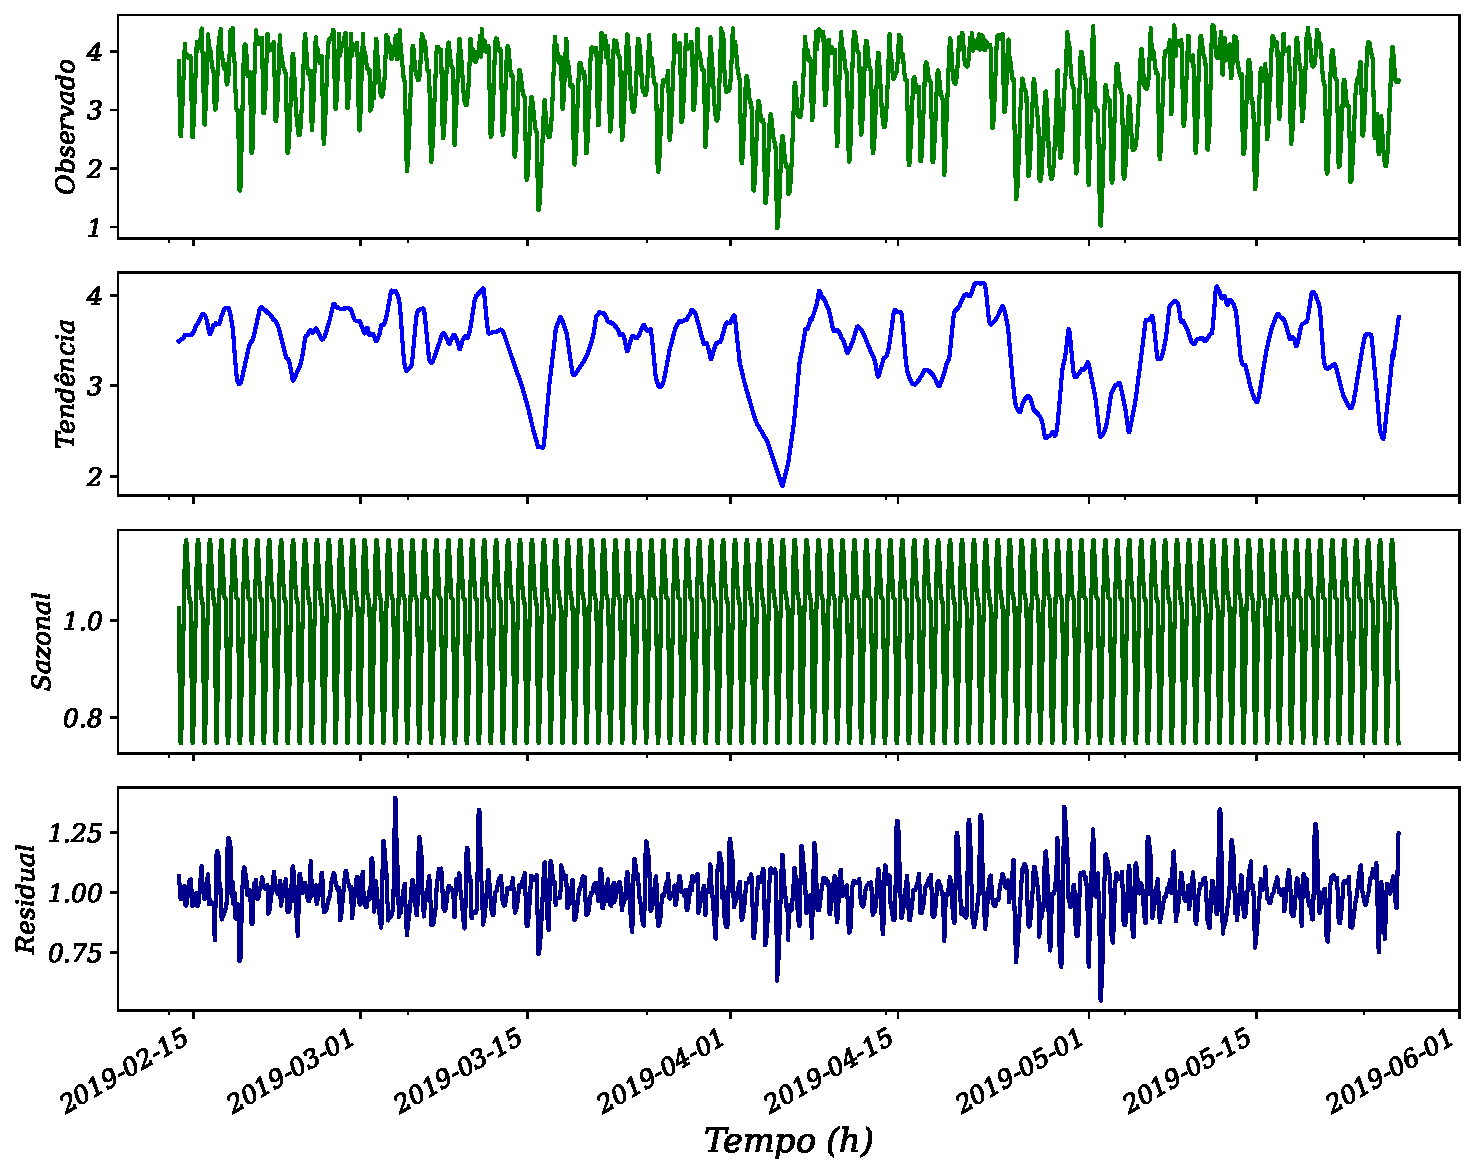
\includegraphics[width=0.8\linewidth]{Resultados/Figuras/STL}
	
	
	
\end{figure}






\textbf{Separa\c c\~ao dos Dados}
na etapa \ref{etp:4}, os dados foram divididos em conjuntos de treinamento, teste e validação. Essa prática é comum entre profissionais de aprendizado de máquina, pois permite avaliar o desempenho do modelo em conjuntos de dados diferentes \cite{raschka2015practical, geron2017hands_on}.

Quanto à divisão dos dados, foi adotada uma estratégia básica em que $70\%$ dos dados foram destinados ao conjunto de treinamento e os $30\%$ restantes foram reservados para o conjunto de teste. Dentro dos $70\%$ de treinamento, foi realizada uma subdivisão em que $80\%$ desses dados foram usados novamente para treinamento e os $20\% $ restantes foram utilizados para validação. Essa abordagem foi implementada em linguagem de programação para facilitar o processo e evitar a necessidade de recalculá-la a cada modificação do modelo.

\textbf{Modelagem e sele\c c\~ao do modelo}
a estratégia recursiva é mencionada por \citeonline{PETROPOULOS2022705} como uma abordagem eficaz na previsão de séries temporais de múltiplos passos. De acordo com o autor, essa estratégia envolve o uso de previsões anteriores como entradas para prever os próximos passos da série temporal. A abordagem recursiva tem demonstrado potencial para melhorar a acurácia das previsões de séries temporais de longo prazo.

Na Etapa \ref{etp:5}, discute-se a previsão dos dados em uma janela de horizonte de previsão estendida, abrangendo diferentes períodos de tempo, como uma hora, seis horas, doze horas e um dia. Essa estratégia de previsão recorrente permite a comparação entre modelos de regressão e modelos ARIMA em diferentes horizontes temporais.

Essa abordagem é vantajosa, pois cada modelo possui suas próprias características e desempenho ao lidar com previsões de curto prazo, como um dia, e previsões de prazo mais longo, como um dia. Ao utilizar uma janela de previsão mais ampla, é possível observar e avaliar melhor as diferenças entre os modelos e analisar seu desempenho em horizontes de tempo variados.

Além desses modelos, vários outros foram implementados no documento, tais como DTR, RFR, XGBRegressor, LGBMRegressor, LSTM, GRU, Prophet, RNN, Transformer, CNN e ANN, a fim de obter o melhor resultado para a previsão de séries temporais de abastecimento de água.

\textbf{Validação e ajuste do modelo}
na etapa \ref{etp:6}, o horizonte de previsão foi personalizado com base no método recursivo de previsão de série temporal e na previsão do nível do tanque LT01. Foram selecionados os seguintes passos para a previsão à frente: uma hora, seis horas, doze horas e um dia. Essa escolha do horizonte de previsão foi feita levando em consideração a estratégia recursiva e os objetivos específicos do estudo. Identifica-se que essa janela de tempo proporciona uma análise mais adequada e comparável entre os modelos utilizados.

Foram utilizados os parâmetros obtidos pelo autoARIMA, que são $(p = 7, d = 0, q = 0) (P = 2, D = 1, Q = 1)_{M = 12}$, mas foram ajustados para obter um melhor resultado, sendo $(p = 7, d = 1, q = 7) (P = 2, D = 1, Q = 1)_{M = 12}$. Na Tabela \ref{tab:autoarima_params}, são exibidos todos os modelos obtidos por esse método do ``autoARIMA'' e ajustados para que obtenham o melhor resultado.
\(p\): Ordem do componente AR (\textit{Auto-Regressivo}),
\(d\): Número de diferenciações não sazonais,
\(q\): Ordem do componente MA (\textit{Média Móvel}),
\(P\): Ordem do componente AR sazonal,
\(D\): Número de diferenciações sazonais,
\(Q\): Ordem do componente MA sazonal,
\(M\): Período sazonal (número de observações em um ciclo sazonal).
Na Tabela \ref{tb:resltsar} mostra como a biblioteca do Python autoARIMA obteve os resultados dos parâmetros, exibindo o STD e os intervalos de confiança nos quais o modelo alcançou o melhor desempenho. O leve ajuste realizado não altera significativamente os parâmetros obtidos nesta biblioteca, permitindo que cada modelo seja trabalhado de maneira eficiente.

\begin{table}[!htb]
	\centering
	\caption{Parâmetros utilizados nos modelos ARIMA e seus antecessores obtidos pelo ``autoARIMA'' do Python.}
	\label{tab:autoarima_params}
	\small
	\begin{tabular}{
			>{\centering\arraybackslash}p{5.5cm}
			>{\centering\arraybackslash}p{6cm}
			>{\centering\arraybackslash}p{3cm}
		}
		\toprule
		\textbf{Modelo} & \textbf{Parâmetros Utilizados} & \textbf{Método de Estimação} \\
		\midrule
		AR(p) & \( p = 7 \) & AutoARIMA \\
		ARX(p) & \( p = 7 \) & AutoARIMA \\
		MA(q) & \( q = 7 \) & AutoARIMA  \\
		ARMA(p, q) & \( p = 7 \), \( q = 7 \) & AutoARIMA  \\
		ARIMA(p, d, q) & \( p = 7 \), \( d = 1 \), \( q = 7 \) & AutoARIMA  \\
		ARIMAX(p, d, q) & \( p = 7 \), \( d = 1 \), \( q = 7 \) & AutoARIMA  \\
		SARIMA(p, d, q)(P, D, Q) & \( p = 7 \), \( d = 1 \), \( q = 7 \), \( P = 2 \), \( D = 1 \), \( Q = 1 \), \( M = 12 \) & AutoARIMA  \\
		SARIMAX(p, d, q)(P, D, Q, M) & \( p = 7 \), \( d = 1 \), \( q = 7 \), \( P = 2 \), \( D = 1 \), \( Q = 1 \), \( M = 12 \) & AutoARIMA  \\
		\bottomrule
	\end{tabular}
\end{table}



\begin{table}[!htb]
	\centering
	\caption{SARIMAX$(7, 0, 0)\times(2, 1, [1], 12)$ Results} \label{tb:resltsar}
	\begin{tabular}{
			l
			S[table-format=1.4]
			S[table-format=1.4]
			S[table-format=3.3]
			S[table-format=1.3]
			S[table-format=1.3]
			S[table-format=1.3]
		}
		\toprule
		& {Coef} & {STD Err} & {z} & {P$>|z|$} & {[0,025} & {0,975]} \\
		\midrule
		Intercept & 0,0003 & 0,000 & 1,053 & 0,292 & -0,000 & 0,001 \\
		ar.L1 & 1,6149 & 0,011 & 141,865 & 0,000 & 1,593 & 1,637 \\
		ar.L2 & -0,8879 & 0,021 & -42,045 & 0,000 & -0,929 & -0,847 \\
		ar.L3 & 0,3167 & 0,024 & 13,033 & 0,000 & 0,269 & 0,364 \\
		ar.L4 & -0,1056 & 0,027 & -3,961 & 0,000 & -0,158 & -0,053 \\
		ar.L5 & -0,1099 & 0,028 & -3,928 & 0,000 & -0,165 & -0,055 \\
		ar.L6 & 0,1431 & 0,027 & 5,368 & 0,000 & 0,091 & 0,195 \\
		ar.L7 & -0,0673 & 0,015 & -4,583 & 0,000 & -0,096 & -0,039 \\
		ar.S.L12 & -0,1222 & 0,016 & -7,705 & 0,000 & -0,153 & -0,091 \\
		ar.S.L24 & 0,1692 & 0,014 & 12,244 & 0,000 & 0,142 & 0,196 \\
		ma.S.L12 & -0,8728 & 0,012 & -74,569 & 0,000 & -0,896 & -0,850 \\
		sigma2 & 0,0157 & 0,000 & 60,022 & 0,000 & 0,015 & 0,016 \\
		\bottomrule
	\end{tabular}
\end{table}


Para os modelos de gradiente \textit{boosting} e redes neurais artificiais, os hiperparâmetros foram otimizados usando a biblioteca Optuna do Python. Nesse contexto, são empregadas técnicas bayesianas, especificamente o algoritmo TPE, visando uma otimização mais eficiente.

Os modelos XGBoost e LightGBM tem como parâmetros e hiperparâmetros mostrado na Tabela \ref{tab:hiperparametros} a otimização dos paramétrios dos modelos XGBoost, LightGBM, RFR e DTR. Esses modelos, devido à sua semelhança, exibem tempos de desempenho próximos um do outro. 



\begin{table}[!htb]
	\centering
	\caption{Hiperparâmetros dos modelos}
	\label{tab:hiperparametros}
	\begin{tabular}{
			>{\centering\arraybackslash}p{2.2cm}
			>{\centering\arraybackslash}p{2.8cm}
			>{\centering\arraybackslash}p{1.9cm}
			>{\centering\arraybackslash}p{1.9cm}
			>{\centering\arraybackslash}p{1.9cm}
			>{\centering\arraybackslash}p{1.9cm}
			>{\centering\arraybackslash}p{1.9cm}
		}
		\toprule
		\textbf{Modelo} & \textbf{Estimadores} & \textbf{Profund. Máxima} & \textbf{Min. Amostras Divisão} & \textbf{Min. Amostras por Folha} & \textbf{Máx. Recursos} & \textbf{Taxa de Aprendizado} \\
		\midrule
		XGB Regressor & 503 & 5 & 7 & 2 & ``sqrt'' & 0,034 \\
		LGBM Regressor & 820 & 10 & 3 & 5 & ``auto'' & 0,014 \\
		Random Forest Regressor & 135 & 10 & 4 & 2 & None & N/A \\
		Decision Tree Regressor & N/A & 229 & 32 & 20 & None & N/A \\
		\bottomrule
	\end{tabular}
\end{table}



Os modelos de rede neural artificial, como RNN, ANN, CNN, GRU, LSTM e Transformer, obtidos na otimização do Optuna do Python, tiveram seus hiperparâmetros melhorados, conforme exibido na Tabela \ref{tab:hyperparameters_summary}. Esses modelos, por serem modelos de rede neural artificial, são melhores para otimizar do que os outros. 

\begin{table}[!htb]
	\centering
	\caption{Resumo dos Hiperparâmetros dos Modelos de Redes Neurais}
	\label{tab:hyperparameters_summary}
	\small
	\begin{tabular}{
			>{\centering\arraybackslash}p{1.8cm}
			>{\centering\arraybackslash}p{2cm}
			>{\centering\arraybackslash}p{2cm}
			>{\centering\arraybackslash}p{2cm}
			>{\centering\arraybackslash}p{2cm}
			>{\centering\arraybackslash}p{1.5cm}
			>{\centering\arraybackslash}p{2.5cm}
		}
		\toprule
		\textbf{Modelo} & \textbf{Unidades/ Layers} & \textbf{Heads/ Dimensões} & \textbf{Tamanho do Batch} & \textbf{Épocas} & \textbf{Dropout/ Learning Rate} & \textbf{Outros Parâmetros} \\
		\midrule
		LSTM & 128 & -- & 32 & 77 & -- & -- \\
		
		GRU & -- & -- & 32 & 50 & -- & -- \\
		
		Transformers & -- & 8 heads, 217; 433 & -- & 50 & -- & 2 camadas \\
		
		RNN & 79 & -- & 16 & 50 & 0,0008612 & -- \\
		
		CNN & -- & -- & 61 & 10 & 0,2799; 0,00052 & Kernel: 7, Densas: 1, Verbosidade: 1 \\
		
		ANN & 125 & -- & 27 & 96 & 0,4135, 0,0004057 & Densas: 1, Verbosidade: 0 \\
		\bottomrule
	\end{tabular}
\end{table}


\textbf{Previs\~ao e avalia\c c\~ao}
a partir da etapa \ref{etp:7}, foram empregadas três métricas amplamente utilizadas na literatura para avaliar e comparar os modelos ARIMA e os modelos de regressão, conforme detalhado na seção \ref{subsec:metrica}.

Na análise dos modelos desenvolvidos, observou-se que o modelo DTR obteve o melhor desempenho, tanto para previsões de curto prazo, durante as horas de pico entre 18h e 21h, quanto para outros períodos. Além disso, os modelos MA, AR, SARIMA, ARIMA, SARIMAX, ARIMAX, ARX, LGBMRegressor, XGBRegressor, RFR, RNN, ANN, CNN, GRU, LSTM, Prophet e Transformer também apresentaram resultados satisfatórios, seguindo uma ordem decrescente de desempenho.

No âmbito das previsões de longo prazo, abrangendo casos de um dia, os modelos ARMA, AR, MA, ARIMA, ARIMAX, ARX, SARIMA, SARIMA, XGBRegressor, RFR, LGBMRegressor, DTR, RNN, ANN, CNN, GRU, LSTM, Prophet e Transformer foram avaliados. Uma observação recorrente foi a superioridade dos modelos que incorporam variáveis exógenas em termos de capacidade de previsão, evidenciada nas Figuras de \ref{fig:1-ar-arx-ma} a \ref{fig:prophet1} e nas Tabelas de \ref{tb:apd-trn} a \ref{tb:apd-int}, onde os valores menores foram destacados em \textbf{negrito} para facilitar a análise. O modelo RNN destacou-se tanto nos conjuntos de treinamento quanto na avaliação global, consolidando-se como o modelo mais eficaz nas previsões realizadas.

Cada figura, desde a \ref{fig:1-ar-arx-ma} até a \ref{fig:prophet1}, ilustra cenários distintos de previsão e comparação entre modelos semelhantes. Os modelos Prophet e RNN, sendo este último a escolha superior, são apresentados de forma isolada. A decisão de não incluir o modelo LR na comparação baseou-se na constância observada em suas previsões a longo prazo.

Ao avaliar os modelos de previsão, tanto nas tabelas quanto nas imagens, o modelo RNN destaca-se como a opção mais eficaz. No caso específico da SANEPAR, esse modelo demonstra um desempenho superior em comparação com os demais modelos de previsão adotados. partir da etapa \ref{etp:7}, três métricas amplamente utilizadas na literatura foram empregadas para avaliar e comparar os modelos ARIMA e os modelos de regressão, conforme detalhado na seção \ref{subsec:metrica}.

Na análise dos modelos desenvolvidos, verificou-se que o modelo DTR alcançou o melhor desempenho, tanto para previsões de curto prazo, durante as horas de pico entre 18h e 21h, quanto para outros períodos. Adicionalmente, os modelos MA, AR, SARIMA, ARIMA, SARIMAX, ARIMAX, ARX, LGBMRegressor, XGBRegressor, RFR, RNN, ANN, CNN, GRU, LSTM, Prophet e Transformer também apresentaram resultados satisfatórios, seguindo uma ordem decrescente de desempenho.

No contexto das previsões de longo prazo, abrangendo períodos de um dia, os modelos ARMA, AR, MA, ARIMA, ARIMAX, ARX, SARIMA, SARIMA, XGBRegressor, RFR, LGBMRegressor, DTR, RNN, ANN, CNN, GRU, LSTM, Prophet e Transformer foram avaliados. Destacou-se a superioridade dos modelos que incorporam variáveis exógenas em termos de capacidade de previsão, evidenciada nas Figuras de \ref{fig:1-ar-arx-ma} a \ref{fig:prophet1} e nas Tabelas de \ref{tb:apd-trn} a \ref{tb:apd-int}, onde os valores menores foram destacados em \textbf{negrito} e \textit{itálico} para facilitar a análise. O modelo RNN destacou-se tanto nos conjuntos de treinamento quanto na avaliação global, consolidando-se como o modelo mais eficaz nas previsões realizadas.

Cada Figura, desde a \ref{fig:1-ar-arx-ma} até a \ref{fig:prophet1}, ilustra cenários distintos de previsão e comparação entre modelos semelhantes. Os modelos Prophet e RNN, sendo este último a escolha superior, são apresentados de forma isolada. A decisão de não incluir o modelo LR na comparação baseou-se na constância observada em suas previsões a longo prazo.

Ao avaliar os modelos de previsão, tanto nas tabelas quanto nas imagens, o modelo RNN destaca-se como a opção mais eficaz. No caso específico da SANEPAR, esse modelo demonstra um desempenho superior em comparação com os demais modelos de previsão adotados.


\begin{figure}[!htb]
	\centering
	\caption{Comparação dos modelos AR, ARX e MA}
	\label{fig:1-ar-arx-ma}
	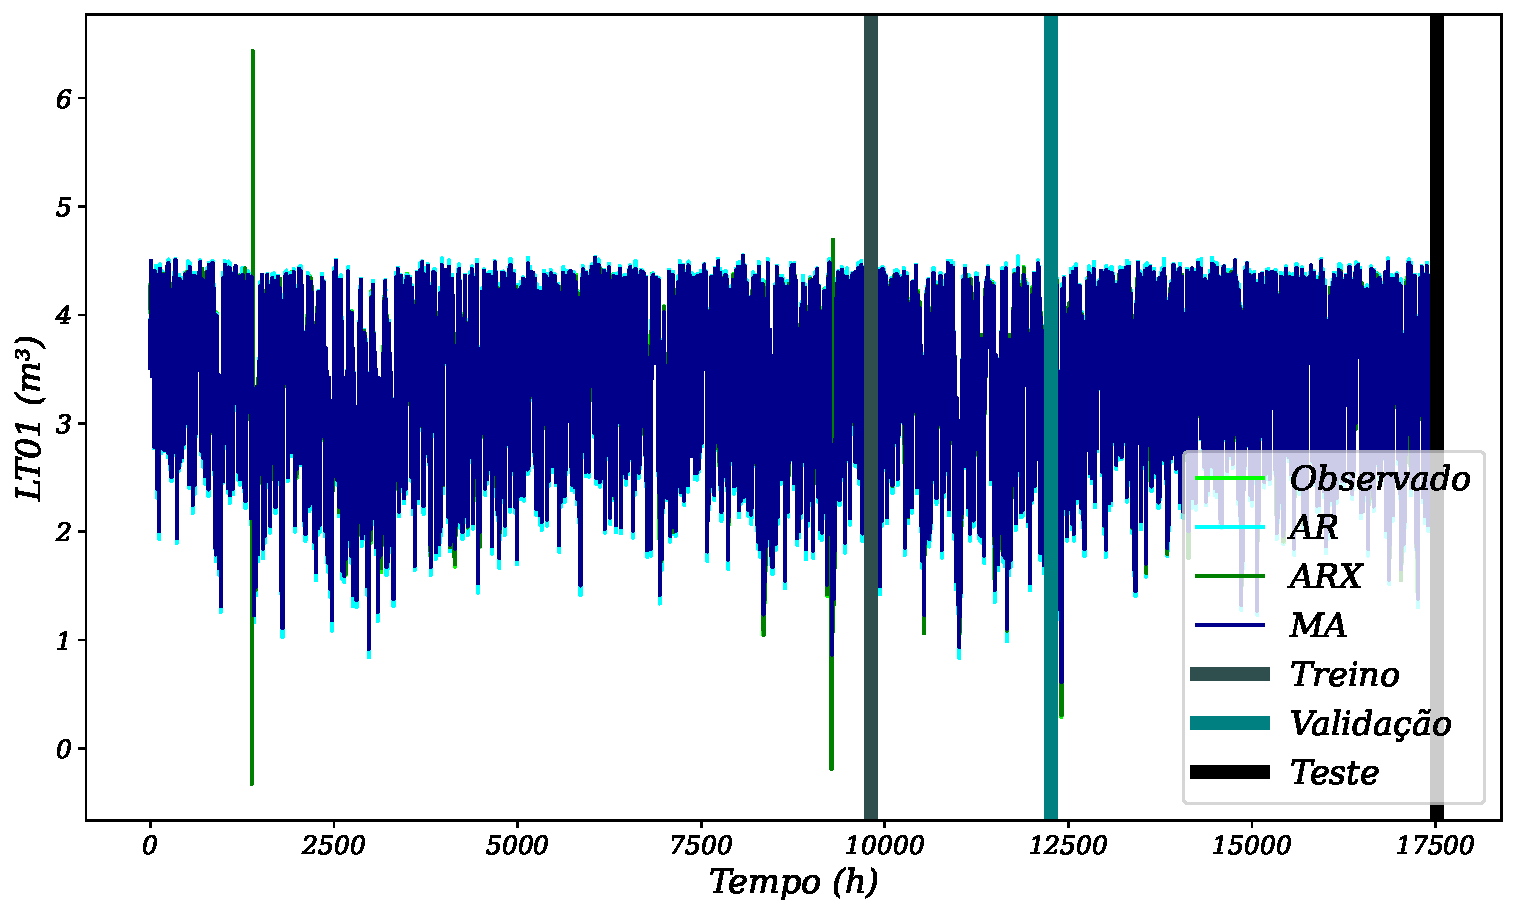
\includegraphics[width=0.6\linewidth]{Resultados/Figuras/1-AR-ARX-MA}
	
\end{figure}
\begin{figure}[!htb]
	\centering
	\caption{Comparação do modelos ARIMAX, SARIMA e SARIMAX}
	\label{fig:1-arimax-sarima-sarimax}
	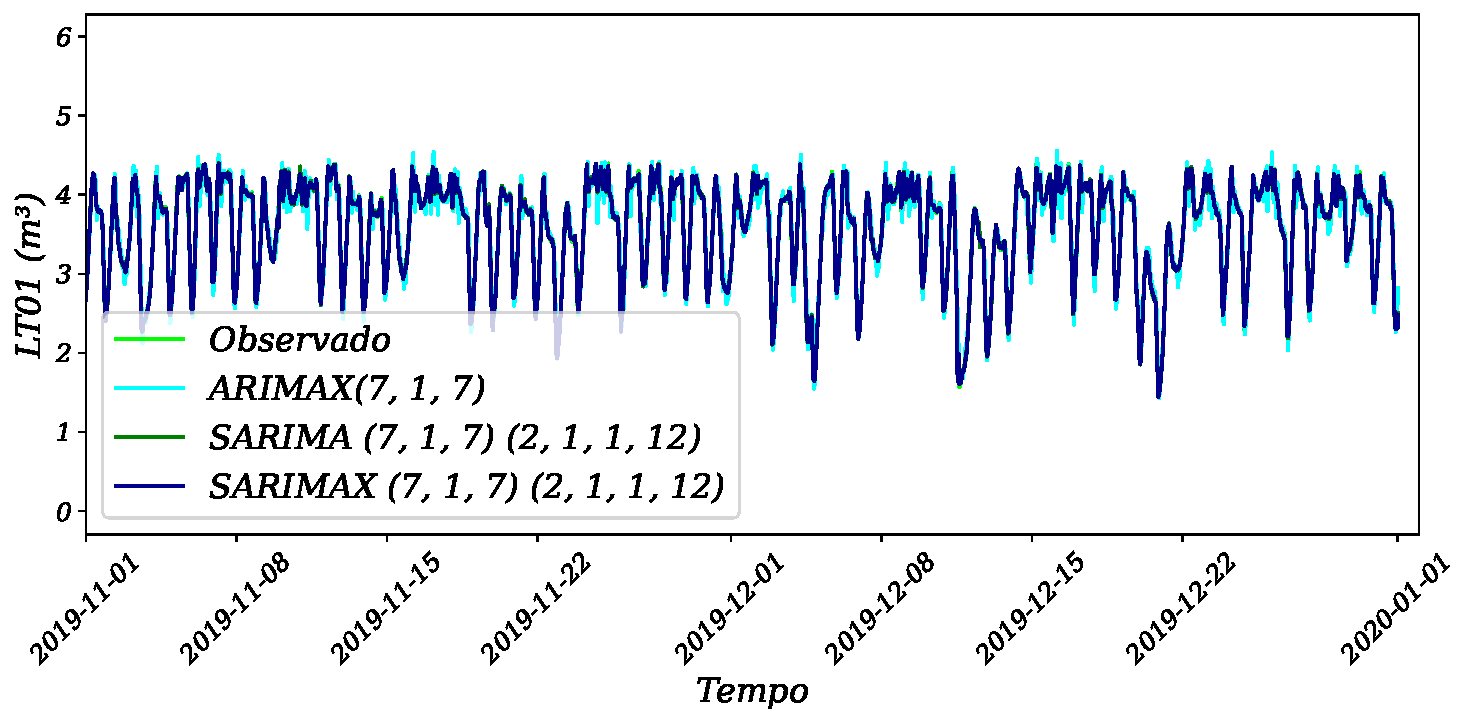
\includegraphics[width=0.6\linewidth]{Resultados/Figuras/1-ARIMAX-SARIMA-SARIMAX}
	
\end{figure}
\begin{figure}[!htb]
	\centering
	\caption{Comparação dos modelos ARMA e ARIMA}
	\label{fig:1-arma-arima}
	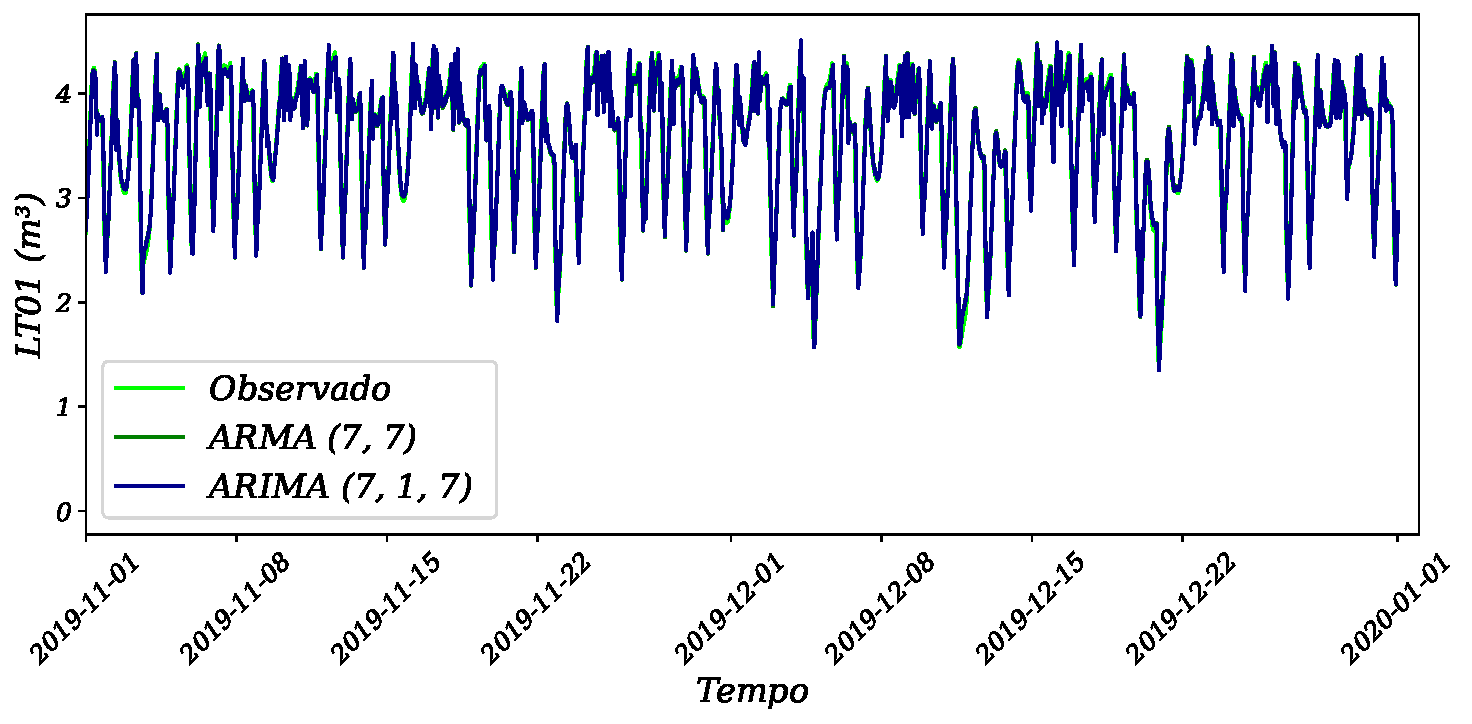
\includegraphics[width=0.6\linewidth]{Resultados/Figuras/1-ARMA-ARIMA}
	
\end{figure}
\begin{figure}[!htb]
	\centering
	\caption{Comparação dos modelos DTR, RFR, XGBoost, Light GBM}
	\label{fig:lr-xgb-lgbm-rf}
	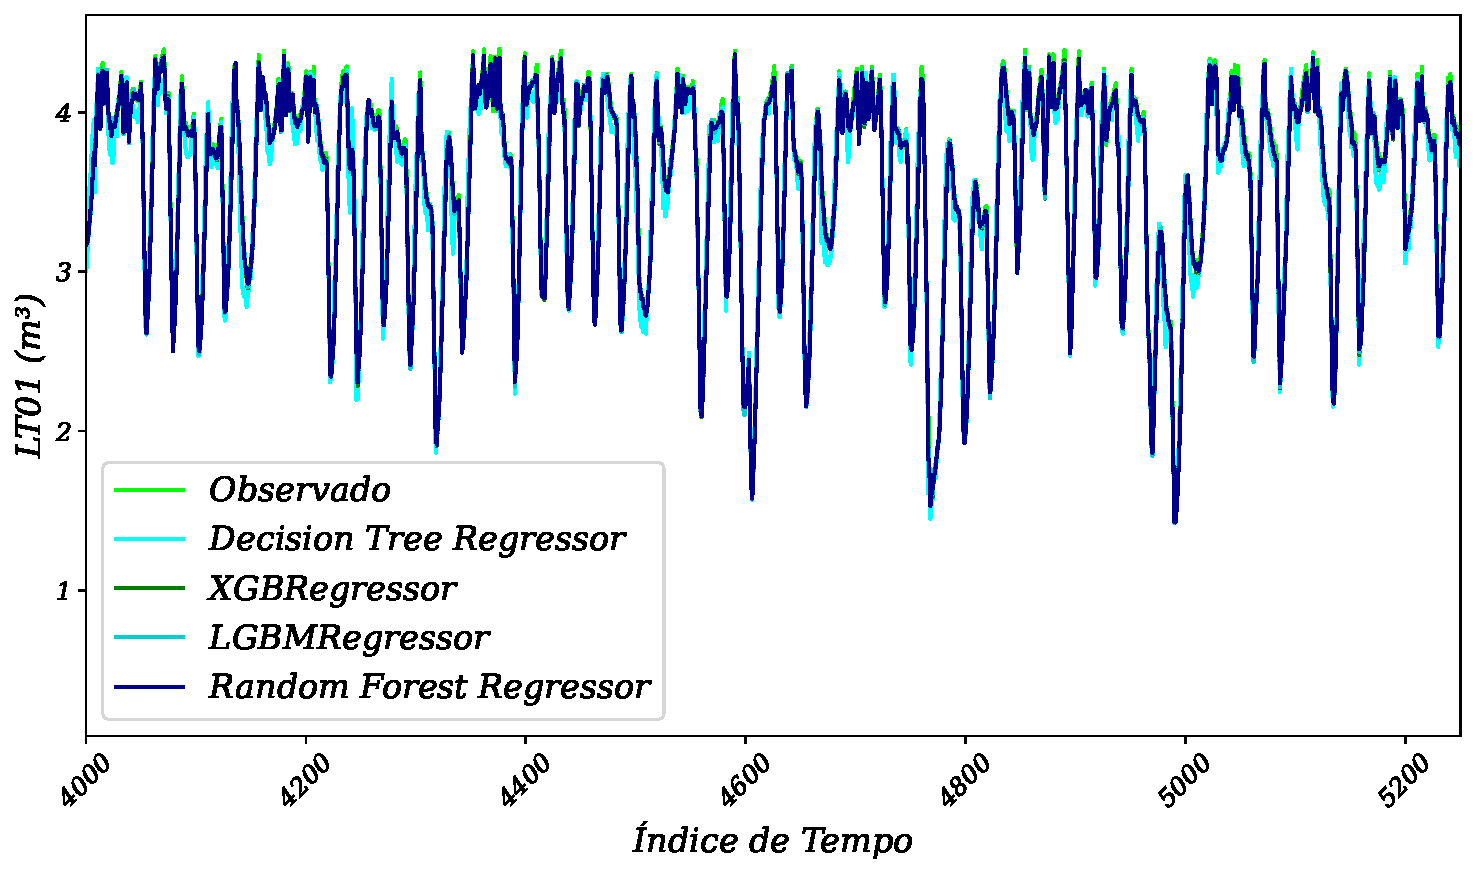
\includegraphics[width=0.6\linewidth]{Resultados/Figuras/LR-XGB-LGBM-RF}
	
\end{figure}
\begin{figure}[!htb]
	\centering
	\caption{Modelo RNN e os vários horizontes }
	\label{fig:rnn}
	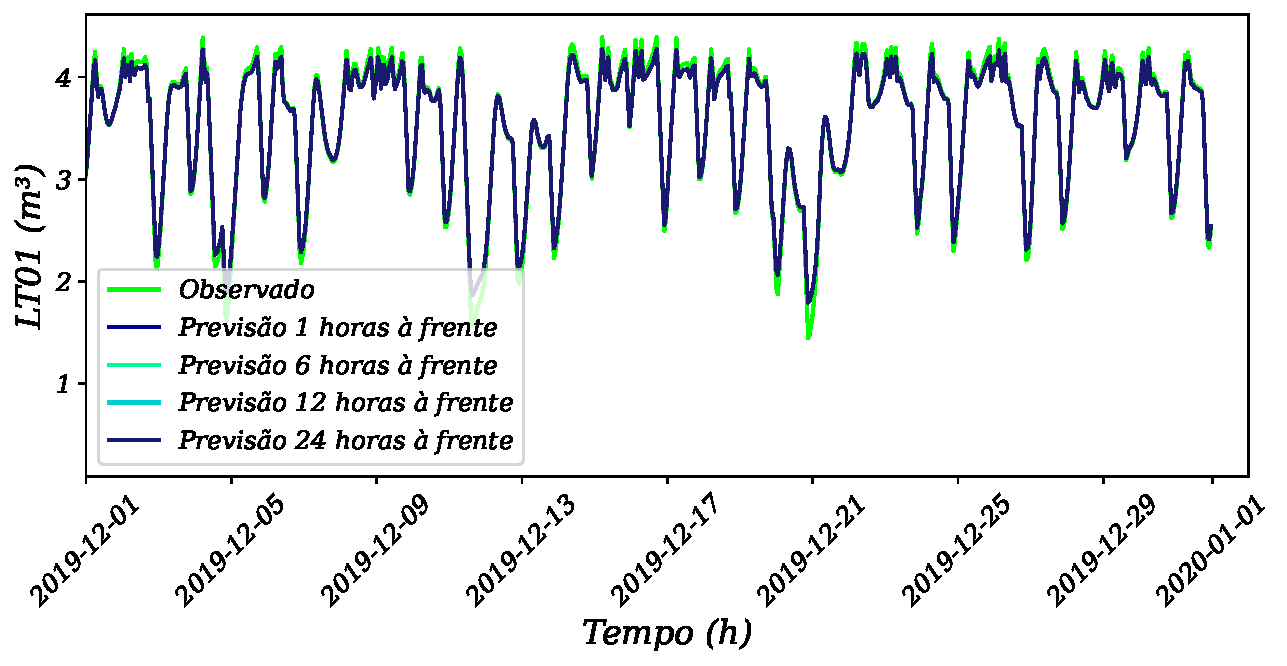
\includegraphics[width=0.6\linewidth]{Resultados/Figuras/RNN}
\end{figure}
\begin{figure}[!htb]
	\centering
	\caption{Previsões do modelo Prophet para o reservatório LT01}\label{fig:prophet1}
	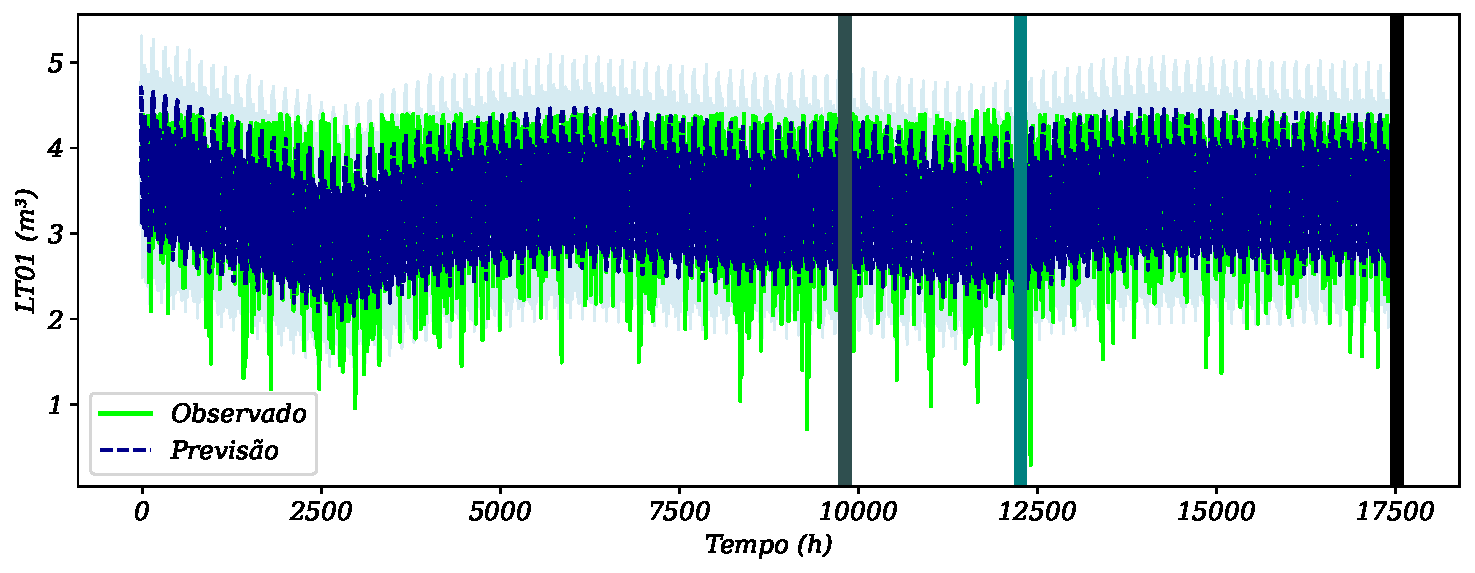
\includegraphics[width=0.7\linewidth]{Resultados/Figuras/prophet1}
	
	
\end{figure}



\begin{landscape}
	
	\begin{table}[!htb]
		\centering
		\small % Reduzir o tamanho da fonte
		\setlength{\tabcolsep}{4pt} % Reduzir o espaçamento entre as colunas
		\caption{Comparação dos modelos de previsão com as métricas de desempenho \textbf{treino}}\label{tb:apd-trn}
		\begin{tabular}{@{}cclllllllllllllllllll@{}}
			\toprule
			&          & \multicolumn{12}{c}{Modelos Treino}                                                                                                                                                                                                                                                           & \multicolumn{1}{c}{\textit{}} & \multicolumn{1}{c}{\textit{}} & \multicolumn{1}{c}{\textit{}} & \multicolumn{1}{c}{\textit{}} & \multicolumn{1}{c}{\textit{}} & \multicolumn{1}{c}{\textit{}} & \multicolumn{1}{c}{\textit{}} \\ \midrule
			Horizontes                         & Métricas & \multicolumn{1}{c}{A} & \multicolumn{1}{c}{B} & \multicolumn{1}{c}{C} & \multicolumn{1}{c}{D} & \multicolumn{1}{c}{E} & \multicolumn{1}{c}{F} & \multicolumn{1}{c}{G} & \multicolumn{1}{c}{H} & \multicolumn{1}{c}{I} & \multicolumn{1}{c}{J} & \multicolumn{1}{c}{K} & \multicolumn{1}{c}{L} & \multicolumn{1}{c}{M}         & \multicolumn{1}{c}{N}         & \multicolumn{1}{c}{O}         & \multicolumn{1}{c}{P}         & \multicolumn{1}{c}{Q}         & \multicolumn{1}{c}{R}         & \multicolumn{1}{c}{S}         \\ \toprule
			\multirow{3}{*}{1 hora à frente}   & sMAPE    & 3,91                  & 4,01                  & 4,03                  & 3,91                  & 3,92                  & 3,89                  & 3,82                  & 3,86                  & 8,85                  & 9,31                  & 9,52                  & 9,37                  & 35,4                          & 35,8                          & 9                             & \textbf{0,0665}               & 16,8                          & 23                            & 23                            \\ 
			& MAE      & \textbf{0,25}         & \textbf{0,25}         & \textbf{0,26}         & \textbf{0,25}         & \textbf{0,25}         & \textbf{0,25}         & \textbf{0,24}         & \textbf{0,25}         & 0,36                  & 0,65                  & 0,67                  & 0,65                  & 1,42                          & 1,44                          & \textbf{0,2}                  & \textit{0,0023}               & 0,55                          & 0,83                          & 0,83                          \\
			& RRMSE    & \textbf{0,09}         & \textbf{0,10}         & \textbf{0,09}         & \textbf{0,09}         & \textbf{0,09}         & \textbf{0,09}         & \textbf{0,09}         & \textbf{0,09}         & \textbf{0,21}         & \textbf{0,21}         & \textbf{0,21}         & \textbf{0,21}         & 2,3                           & 0,65                          & \textbf{0,2}                  & \textit{0,0008}               & 0,31                          & 0,48                          & 0,48                          \\ \toprule
			\multirow{3}{*}{6 horas à frente}  & sMAPE    & 9,97                  & 10,1                  & 9,7                   & 9,98                  & 9,97                  & 10                    & 10,1                  & 9,99                  & 6,99                  & 12,4                  & 12,7                  & 9,369                 & 66,2                          & 83,9                          & 20                            & \textit{0,0230}               & 16,7                          & 20,6                          & 20,6                          \\
			& MAE      & 0,64                  & 0,65                  & 0,62                  & 0,64                  & 0,64                  & 0,64                  & 0,65                  & 0,64                  & 0,59                  & 0,9                   & 0,93                  & 0,651                 & 3,37                          & 4,95                          & 0,6                           & \textit{0,0007}               & 0,55                          & 0,72                          & 0,72                          \\
			& RRMSE    & \textbf{0,23}         & \textbf{0,23}         & \textbf{0,23}         & \textbf{0,23}         & \textbf{0,23}         & \textbf{0,23}         & \textbf{0,23}         & \textbf{0,23}         & \textbf{0,16}         & 0,32                  & 0,33                  & \textbf{0,209}        & 5,02                          & 1,71                          & 0,6                           & \textit{0,0006}               & 0,31                          & 0,45                          & 0,45                          \\ \toprule
			\multirow{3}{*}{12 horas à frente} & sMAPE    & 11,6                  & 11,6                  & 11,3                  & 11,6                  & 11,5                  & 11,7                  & 11,8                  & 11,6                  & 6,99                  & 12,4                  & 12,7                  & 9,369                 & 72                            & 98,6                          & 25                            & \textbf{0,0683}               & 16,8                          & 29,2                          & 29,2                          \\
			& MAE      & 0,75                  & 0,75                  & 0,74                  & 0,75                  & 0,75                  & 0,76                  & 0,77                  & 0,75                  & 0,59                  & 0,9                   & 0,93                  & 0,651                 & 3,83                          & 6,69                          & 0,8                           & \textit{0,0022}               & 0,55                          & 1,11                          & 1,11                          \\
			& RRMSE    & \textbf{0,27}         & \textbf{0,27}         & \textbf{0,26}         & \textbf{0,27}         & \textbf{0,26}         & \textbf{0,27}         & \textbf{0,27}         & \textbf{0,27}         & \textbf{0,16}         & 0,32                  & 0,33                  & \textbf{0,209}        & 5,69                          & 2,25                          & 0,9                           & \textit{0,0009}               & 0,31                          & 0,55                          & 0,55                          \\ \toprule
			\multirow{3}{*}{24 horas à frente} & sMAPE    & 6,77                  & 6,85                  & 6,67                  & 6,77                  & 6,69                  & 6,82                  & 6,86                  & 6,82                  & 6,99                  & 12,4                  & 12,7                  & 9,369                 & 74,4                          & 104                           & 26                            & \textbf{0,2328}               & 16,8                          & 26,8                          & 26,8                          \\
			& MAE      & 0,43                  & 0,44                  & 0,43                  & 0,43                  & 0,43                  & 0,44                  & 0,44                  & 0,43                  & 0,59                  & 0,9                   & 0,93                  & 0,651                 & 4,04                          & 7,5                           & 0,8                           & \textit{0,0079}               & 0,55                          & 1                             & 1                             \\
			& RRMSE    & \textbf{0,17}         & \textbf{0,17}         & \textbf{0,17}         & \textbf{0,17}         & \textbf{0,17}         & \textbf{0,17}         & \textbf{0,17}         & \textbf{0,17}         & \textbf{0,16}         & 0,32                  & 0,33                  & \textbf{0,209}        & 5,99                          & 2,5                           & 1                             & \textit{0,0024}               & 0,31                          & 0,52                          & 0,52                          \\ \cmidrule(l){1-21} 				
		\end{tabular}
		
		\captionsetup{justification=centering} % Centralizar a legenda
		Legenda para os Modelos de Previsão: A - AR, B - ARX, C - MA, D - ARMA, E - ARIMA, F - SARIMA, G - ARIMAX, H - SARIMAX, I - Decision Tree Regressor, J - Random Forest Regressor, K - XGBRegressor, L - LGBMRegressor, M - LSTM, N - GRU, O - Prophet, P - RNN, Q - Transformer, R - CNN, S - ANN.
	\end{table}
	
	\newpage
	
	\begin{table}[!htb]
		\centering
		\small % Reduzir o tamanho da fonte
		\setlength{\tabcolsep}{4pt} % Reduzir o espaçamento entre as colunas
		\caption{Comparação dos modelos de previsão com as métricas de desempenho \textbf{teste}}\label{tb:apd-tst}
		\begin{tabular}{@{}cclllllllllllllllllll@{}}
			\toprule
			&          & \multicolumn{12}{c}{Modelos Teste}                                                                                                                                                                                                                                                            & \multicolumn{1}{c}{\textit{}} & \multicolumn{1}{c}{\textit{}} & \multicolumn{1}{c}{\textit{}} & \multicolumn{1}{c}{\textit{}} & \multicolumn{1}{c}{\textit{}} & \multicolumn{1}{c}{\textit{}} & \multicolumn{1}{c}{\textit{}} \\ \midrule
			Horizontes                         & Métricas & \multicolumn{1}{c}{A} & \multicolumn{1}{c}{B} & \multicolumn{1}{c}{C} & \multicolumn{1}{c}{D} & \multicolumn{1}{c}{E} & \multicolumn{1}{c}{F} & \multicolumn{1}{c}{G} & \multicolumn{1}{c}{H} & \multicolumn{1}{c}{I} & \multicolumn{1}{c}{J} & \multicolumn{1}{c}{K} & \multicolumn{1}{c}{L} & \multicolumn{1}{c}{M}         & \multicolumn{1}{c}{N}         & \multicolumn{1}{c}{O}         & \multicolumn{1}{c}{P}         & \multicolumn{1}{c}{Q}         & \multicolumn{1}{c}{R}         & \multicolumn{1}{c}{S}         \\ \toprule
			\multirow{3}{*}{1 hora à frente}   & sMAPE    & 3,93                  & 4,15                  & 3,99                  & 3,93                  & 3,92                  & 3,91                  & 4,16                  & 4,16                  & 7,76                  & 8,46                  & 8,68                  & 8,45                  & 15,6                          & 15,9                          & 9                             & \textbf{0,0744}               & 15,1                          & 20,6                          & 20,6                          \\
			& MAE      & \textbf{0,26}         & \textbf{0,27}         & \textbf{0,26}         & \textbf{0,26}         & \textbf{0,26}         & \textbf{0,26}         & \textbf{0,27}         & \textbf{0,27}         & 0,40                  & 0,61                  & 0,63                  & 0,61                  & 0,53                          & 0,54                          & \textbf{0,2}                  & \textit{0,0024}               & 0,52                          & 0,76                          & 0,76                          \\
			& RRMSE    & \textbf{0,09}         & \textbf{0,10}         & \textbf{0,09}         & \textbf{0,09}         & \textbf{0,09}         & \textbf{0,09}         & \textbf{0,10}         & \textbf{0,10}         & \textbf{0,18}         & \textbf{0,19}         & \textbf{0,20}         & \textbf{0,19}         & 1,01                          & 0,33                          & \textbf{0,2}                  & \textit{0,0029}               & 0,34                          & 0,5                           & 0,5                           \\ \toprule
			\multirow{3}{*}{6 horas à frente}  & sMAPE    & 9,74                  & 9,94                  & 9,44                  & 9,74                  & 9,71                  & 9,76                  & 9,96                  & 9,96                  & 6,36                  & 10,7                  & 11                    & 8,446                 & 59,5                          & 72,7                          & 20                            & \textit{0,0308}               & 15,1                          & 17,3                          & 17,3                          \\
			& MAE      & 0,65                  & 0,66                  & 0,63                  & 0,65                  & 0,65                  & 0,65                  & 0,66                  & 0,66                  & 0,56                  & 0,8                   & 0,82                  & 0,609                 & 2,97                          & 4,04                          & 0,6                           & \textit{0,0007}               & 0,51                          & 0,62                          & 0,62                          \\
			& RRMSE    & \textbf{0,23}         & \textbf{0,23}         & \textbf{0,22}         & \textbf{0,23}         & \textbf{0,23}         & \textbf{0,23}         & \textbf{0,23}         & \textbf{0,23}         & \textbf{0,14}         & \textbf{0,28}         & \textbf{0,29}         & \textbf{0,191}        & 4,9                           & 1,42                          & 0,6                           & \textit{0,0033}               & 0,34                          & 0,46                          & 0,46                          \\ \toprule
			\multirow{3}{*}{12 horas à frente} & sMAPE    & 11,1                  & 11,2                  & 10,9                  & 11,1                  & 11,1                  & 11,2                  & 11,2                  & 11,3                  & 6,36                  & 10,8                  & 11                    & 8,446                 & 68,4                          & 94,1                          & 25                            & \textbf{0,0745}               & 15,1                          & 18,8                          & 18,8                          \\
			& MAE      & 0,74                  & 0,75                  & 0,73                  & 0,74                  & 0,74                  & 0,75                  & 0,75                  & 0,75                  & 0,56                  & 0,8                   & 0,82                  & 0,609                 & 3,67                          & 6,31                          & 0,8                           & \textit{0,0023}               & 0,52                          & 0,68                          & 0,68                          \\
			& RRMSE    & \textbf{0,26}         & \textbf{0,26}         & \textbf{0,25}         & \textbf{0,26}         & \textbf{0,26}         & \textbf{0,26}         & \textbf{0,26}         & \textbf{0,26}         & \textbf{0,14}         & \textbf{0,28}         & \textbf{0,29}         & \textbf{0,191}        & 6,01                          & 2,11                          & 0,9                           & \textit{0,0032}               & 0,34                          & 0,48                          & 0,48                          \\ \toprule
			\multirow{3}{*}{24 horas à frente} & sMAPE    & 6,15                  & 6,34                  & 6,08                  & 6,15                  & 6,14                  & 6,24                  & 6,36                  & 6,37                  & 6,36                  & 10,7                  & 11                    & 8,446                 & 71,5                          & 102                           & 26                            & \textbf{0,2385}               & 15,1                          & 18,1                          & 18,1                          \\
			& MAE      & 0,4                   & 0,41                  & 0,4                   & 0,4                   & 0,4                   & 0,41                  & 0,42                  & 0,42                  & 0,56                  & 0,8                   & 0,83                  & 0,609                 & 3,92                          & 7,36                          & 0,8                           & \textit{0,0081}               & 0,52                          & 0,65                          & 0,65                          \\
			& RRMSE    & \textbf{0,16}         & \textbf{0,16}         & \textbf{0,16}         & \textbf{0,16}         & \textbf{0,16}         & \textbf{0,16}         & \textbf{0,16}         & \textbf{0,16}         & \textbf{0,14}         & \textbf{0,28}         & \textbf{0,29}         & \textbf{0,191}        & 6,42                          & 2,43                          & 1                             & \textit{0,0041}               & 0,34                          & 0,47                          & 0,47                          \\ \cmidrule(l){1-21} 
		\end{tabular}
		
		\captionsetup{justification=centering} % Centralizar a legenda
		Legenda para os Modelos de Previsão: A - AR, B - ARX, C - MA, D - ARMA, E - ARIMA, F - SARIMA, G - ARIMAX, H - SARIMAX, I - Decision Tree Regressor, J - Random Forest Regressor, K - XGBRegressor, L - LGBMRegressor, M - LSTM, N - GRU, O - Prophet, P - RNN, Q - Transformer, R - CNN, S - ANN.
	\end{table}
	
	\newpage
	
	\begin{table}[!htb]
		\centering
		\small % Reduzir o tamanho da fonte
		\setlength{\tabcolsep}{4pt} % Reduzir o espaçamento entre as colunas
		\caption{Comparação dos modelos de previsão com as métricas de desempenho \textbf{validação}}\label{tb:apd-vld}
		\begin{tabular}{@{}cclllllllllllllllllll@{}}
			\toprule
			&          & \multicolumn{12}{c}{Modelos Validação}                                                                                                                                                                                                                                                        & \multicolumn{1}{c}{\textit{}} & \multicolumn{1}{c}{\textit{}} & \multicolumn{1}{c}{\textit{}} & \multicolumn{1}{c}{\textit{}} & \multicolumn{1}{c}{\textit{}} & \multicolumn{1}{c}{\textit{}} & \multicolumn{1}{c}{\textit{}} \\ \midrule
			Horizontes                         & Métricas & \multicolumn{1}{c}{A} & \multicolumn{1}{c}{B} & \multicolumn{1}{c}{C} & \multicolumn{1}{c}{D} & \multicolumn{1}{c}{E} & \multicolumn{1}{c}{F} & \multicolumn{1}{c}{G} & \multicolumn{1}{c}{H} & \multicolumn{1}{c}{I} & \multicolumn{1}{c}{J} & \multicolumn{1}{c}{K} & \multicolumn{1}{c}{L} & \multicolumn{1}{c}{M}         & \multicolumn{1}{c}{N}         & \multicolumn{1}{c}{O}         & \multicolumn{1}{c}{P}         & \multicolumn{1}{c}{Q}         & \multicolumn{1}{c}{R}         & \multicolumn{1}{c}{S}         \\ \toprule
			\multirow{3}{*}{1 hora à frente}   & sMAPE    & 4,08                  & 4,28                  & 4,20                  & 4,09                  & 4,10                  & 4,20                  & 4,26                  & 4,29                  & 8,54                  & 10,47                 & 10,66                 & 10,45                 & 29,8                          & 29,4                          & 9                             & \textbf{0,0675}               & 17,4                          & 18,3                          & 18,3                          \\
			& MAE      & \textbf{0,25}         & \textbf{0,26}         & \textbf{0,26}         & \textbf{0,25}         & \textbf{0,25}         & \textbf{0,26}         & \textbf{0,26}         & \textbf{0,26}         & 0,32                  & 0,72                  & 0,74                  & 0,72                  & 1,1                           & 1,08                          & \textbf{0,2}                  & \textit{0,0023}               & 0,56                          & 0,6                           & 0,6                           \\
			& RRMSE    & \textbf{0,10}         & \textbf{0,10}         & \textbf{0,10}         & \textbf{0,10}         & \textbf{0,10}         & \textbf{0,10}         & \textbf{0,10}         & \textbf{0,10}         & \textbf{0,20}         & \textbf{0,23}         & \textbf{0,24}         & \textbf{0,23}         & 1,87                          & 0,56                          & \textbf{0,2}                  & \textit{0,0008}               & 0,33                          & 0,39                          & 0,39                          \\ \toprule
			\multirow{3}{*}{6 horas à frente}  & sMAPE    & 10,9                  & 11,1                  & 10,6                  & 10,9                  & 10,9                  & 11                    & 11,1                  & 11,1                  & 6,8                   & 13,9                  & 14,2                  & 10,45                 & 67,9                          & 84                            & 20                            & \textit{0,0229}               & 17,4                          & 20,5                          & 20,5                          \\
			& MAE      & 0,68                  & 0,69                  & 0,66                  & 0,68                  & 0,68                  & 0,69                  & 0,69                  & 0,69                  & 0,57                  & 1,01                  & 1,04                  & 0,721                 & 3,39                          & 4,81                          & 0,6                           & \textit{0,0007}               & 0,56                          & 0,69                          & 0,69                          \\
			& RRMSE    & \textbf{0,25}         & \textbf{0,25}         & \textbf{0,24}         & \textbf{0,25}         & \textbf{0,25}         & \textbf{0,25}         & \textbf{0,25}         & \textbf{0,25}         & \textbf{0,16}         & \textbf{0,36}         & \textbf{0,37}         & \textbf{0,233}        & 4,98                          & 1,72                          & 0,6                           & \textit{0,0005}               & 0,34                          & 0,44                          & 0,44                          \\ \toprule
			\multirow{3}{*}{12 horas à frente} & sMAPE    & 12,7                  & 12,8                  & 12,4                  & 12,7                  & 12,6                  & 12,8                  & 12,8                  & 12,8                  & 6,8                   & 13,9                  & 14,2                  & 10,45                 & 74,4                          & 100                           & 25                            & \textbf{0,0689}               & 17,4                          & 22,9                          & 22,9                          \\
			& MAE      & 0,8                   & 0,81                  & 0,79                  & 0,8                   & 0,8                   & 0,81                  & 0,81                  & 0,81                  & 0,57                  & 1,01                  & 1,04                  & 0,721                 & 3,92                          & 6,71                          & 0,8                           & \textit{0,0022}               & 0,56                          & 0,79                          & 0,79                          \\
			& RRMSE    & \textbf{0,29}         & \textbf{0,29}         & \textbf{0,28}         & \textbf{0,29}         & \textbf{0,29}         & \textbf{0,29}         & \textbf{0,29}         & \textbf{0,29}         & \textbf{0,16}         & \textbf{0,36}         & \textbf{0,37}         & \textbf{0,233}        & 5,73                          & 2,33                          & 0,9                           & \textit{0,0008}               & 0,33                          & 0,48                          & 0,48                          \\ \toprule
			\multirow{3}{*}{24 horas à frente} & sMAPE    & 7,3                   & 7,45                  & 7,19                  & 7,3                   & 7,27                  & 7,37                  & 7,43                  & 7,46                  & 6,8                   & 13,9                  & 14,2                  & 10,45                 & 76,9                          & 106                           & 26                            & \textbf{0,2342}               & 17,4                          & 22,9                          & 22,9                          \\
			& MAE      & 0,46                  & 0,46                  & 0,45                  & 0,46                  & 0,45                  & 0,46                  & 0,46                  & 0,46                  & 0,57                  & 1,01                  & 1,04                  & 0,721                 & 4,14                          & 7,59                          & 0,8                           & \textit{0,0077}               & 0,56                          & 0,79                          & 0,79                          \\
			& RRMSE    & \textbf{0,18}         & \textbf{0,18}         & \textbf{0,18}         & \textbf{0,18}         & \textbf{0,18}         & \textbf{0,18}         & \textbf{0,18}         & \textbf{0,18}         & \textbf{0,16}         & \textbf{0,36}         & \textbf{0,37}         & \textbf{0,233}        & 6,04                          & 2,61                          & 1                             & \textit{0,0024}               & 0,33                          & 0,48                          & 0,48                          \\ \cmidrule(l){1-21} 
		\end{tabular}
		
		\captionsetup{justification=centering} % Centralizar a legenda
		Legenda para os Modelos de Previsão: A - AR, B - ARX, C - MA, D - ARMA, E - ARIMA, F - SARIMA, G - ARIMAX, H - SARIMAX, I - Decision Tree Regressor, J - Random Forest Regressor, K - XGBRegressor, L - LGBMRegressor, M - LSTM, N - GRU, O - Prophet, P - RNN, Q - Transformer, R - CNN, S - ANN.
	\end{table}
	
	\newpage
	
	\begin{table}[!htb]
		\centering
		\small % Reduzir o tamanho da fonte
		\setlength{\tabcolsep}{4pt} % Reduzir o espaçamento entre as colunas
		\caption{Comparação dos modelos de previsão com as métricas de desempenho \textbf{inteiro}}\label{tb:apd-int}
		\begin{tabular}{@{}cclllllllllllllllllll@{}}
			\toprule
			&          & \multicolumn{12}{c}{Modelos Inteiros}                                                                                                                                                                                                                                                         & \multicolumn{1}{c}{\textit{}} & \multicolumn{1}{c}{\textit{}} & \multicolumn{1}{c}{\textit{}} & \multicolumn{1}{c}{\textit{}} & \multicolumn{1}{c}{\textit{}} & \multicolumn{1}{c}{\textit{}} & \multicolumn{1}{c}{\textit{}} \\ \midrule
			Horizontes                         & Métricas & \multicolumn{1}{c}{A} & \multicolumn{1}{c}{B} & \multicolumn{1}{c}{C} & \multicolumn{1}{c}{D} & \multicolumn{1}{c}{E} & \multicolumn{1}{c}{F} & \multicolumn{1}{c}{G} & \multicolumn{1}{c}{H} & \multicolumn{1}{c}{I} & \multicolumn{1}{c}{J} & \multicolumn{1}{c}{K} & \multicolumn{1}{c}{L} & \multicolumn{1}{c}{M}         & \multicolumn{1}{c}{N}         & \multicolumn{1}{c}{O}         & \multicolumn{1}{c}{P}         & \multicolumn{1}{c}{Q}         & \multicolumn{1}{c}{R}         & \multicolumn{1}{c}{S}         \\ \toprule
			\multirow{3}{*}{1 hora à frente}   & sMAPE    & 3,94                  & 4,08                  & 4,05                  & 3,93                  & 3,95                  & 3,91                  & 4,05                  & 4,05                  & 8,51                  & 9,22                  & 9,43                  & 9,244                 & 17,1                          & 17,4                          & 9                             & \textbf{0,0690}               & 16,4                          & 22,5                          & 22,5                          \\
			& MAE      & \textbf{0,25}         & \textbf{0,26}         & \textbf{0,26}         & \textbf{0,25}         & \textbf{0,25}         & \textbf{0,25}         & \textbf{0,26}         & \textbf{0,26}         & 0,36                  & 0,65                  & 0,67                  & 0,648                 & 0,57                          & 0,58                          & \textbf{0,2}                  & \textit{0,0023}               & 0,54                          & 0,81                          & 0,81                          \\
			& RRMSE    & \textbf{0,09}         & \textbf{0,1}          & \textbf{0,09}         & \textbf{0,09}         & \textbf{0,09}         & \textbf{0,09}         & \textbf{0,1}          & \textbf{0,1}          & \textbf{0,2}          & \textbf{0,21}         & \textbf{0,21}         & \textbf{0,207}        & 1,01                          & 0,31                          & \textbf{0,2}                  & \textit{0,0017}               & 0,32                          & 0,49                          & 0,49                          \\ \toprule
			\multirow{3}{*}{6 horas à frente}  & sMAPE    & 10                    & 10,2                  & 9,75                  & 10                    & 10                    & 10,1                  & 10,2                  & 10,1                  & 6,77                  & 12,1                  & 12,4                  & 12,07                 & 61,7                          & 74,6                          & 20                            & \textit{0,0253}               & 16,3                          & 20                            & 20                            \\
			& MAE      & 0,65                  & 0,66                  & 0,63                  & 0,65                  & 0,65                  & 0,65                  & 0,66                  & 0,65                  & 0,58                  & 0,89                  & 0,91                  & 0,885                 & 3,04                          & 4,08                          & 0,6                           & \textit{0,0007}               & 0,54                          & 0,7                           & 0,7                           \\
			& RRMSE    & \textbf{0,23}         & \textbf{0,23}         & \textbf{0,23}         & \textbf{0,23}         & \textbf{0,23}         & \textbf{0,23}         & \textbf{0,23}         & \textbf{0,23}         & \textbf{0,16}         & \textbf{0,32}         & \textbf{0,32}         & \textbf{0,316}        & 4,65                          & 1,45                          & 0,6                           & \textit{0,0019}               & 0,33                          & 0,46                          & 0,46                          \\ \toprule
			\multirow{3}{*}{12 horas à frente} & sMAPE    & 11,6                  & 11,7                  & 11,4                  & 11,6                  & 11,6                  & 11,7                  & 11,8                  & 11,7                  & 6,77                  & 12,1                  & 12,4                  & 12,12                 & 70,7                          & 96                            & 25                            & \textbf{0,0703}               & 16,4                          & 28,7                          & 28,7                          \\
			& MAE      & 0,76                  & 0,76                  & 0,74                  & 0,76                  & 0,75                  & 0,76                  & 0,77                  & 0,76                  & 0,58                  & 0,89                  & 0,91                  & 0,889                 & 3,75                          & 6,38                          & 0,8                           & \textit{0,0023}               & 0,54                          & 1,09                          & 1,09                          \\
			& RRMSE    & \textbf{0,27}         & \textbf{0,27}         & \textbf{0,26}         & \textbf{0,27}         & \textbf{0,27}         & \textbf{0,27}         & \textbf{0,27}         & \textbf{0,27}         & \textbf{0,16}         & \textbf{0,32}         & \textbf{0,32}         & \textbf{0,317}        & 5,69                          & 2,16                          & 0,9                           & \textit{0,0019}               & 0,32                          & 0,56                          & 0,56                          \\ \toprule
			\multirow{3}{*}{24 horas à frente} & sMAPE    & 6,66                  & 6,79                  & 6,57                  & 6,66                  & 6,6                   & 6,71                  & 6,82                  & 6,8                   & 6,77                  & 12,1                  & 12,4                  & 12,21                 & 73,8                          & 104                           & 26                            & \textbf{0,2347}               & 16,4                          & 26,2                          & 26,2                          \\
			& MAE      & 0,43                  & 0,43                  & 0,42                  & 0,43                  & 0,42                  & 0,43                  & 0,44                  & 0,43                  & 0,58                  & 0,89                  & 0,92                  & 0,897                 & 4,01                          & 7,44                          & 0,8                           & \textit{0,0080}               & 0,54                          & 0,98                          & 0,98                          \\
			& RRMSE    & \textbf{0,17}         & \textbf{0,17}         & \textbf{0,17}         & \textbf{0,17}         & \textbf{0,17}         & \textbf{0,17}         & \textbf{0,17}         & \textbf{0,17}         & \textbf{0,16}         & \textbf{0,32}         & \textbf{0,32}         & \textbf{0,319}        & 6,07                          & 2,49                          & 1                             & \textit{0,0030}               & 0,32                          & 0,53                          & 0,53                          \\ \cmidrule(l){1-21} 
		\end{tabular}
		
		\captionsetup{justification=centering} % Centralizar a legenda
		Legenda para os Modelos de Previsão: A - AR, B - ARX, C - MA, D - ARMA, E - ARIMA, F - SARIMA, G - ARIMAX, H - SARIMAX, I - Decision Tree Regressor, J - Random Forest Regressor, K - XGBRegressor, L - LGBMRegressor, M - LSTM, N - GRU, O - Prophet, P - RNN, Q - Transformer, R - CNN, S - ANN.
	\end{table}
	
\end{landscape}

\textbf{Teste de signific\^ancia}
na etapa \ref{etp:8}, realizou-se o teste de Friedman e o teste de Nemenyi para comparar as classificações médias entre os diversos classificadores. O teste de Nemenyi é uma ferramenta de comparação múltipla frequentemente empregada após a aplicação de testes não paramétricos com três ou mais fatores.

A matriz de comparação entre os classificadores, apresentada na Tabela \ref{tb:nemeyi}, exibe os valores de comparação múltipla de Nemenyi, onde as entradas evidenciam as diferenças significativas entre os pares de classificadores.

A Tabela \ref{tb:nemeyi} apresenta os resultados do teste de Nemenyi, um método utilizado para comparar as classificações médias entre diferentes classificadores após a aplicação de testes não paramétricos com três ou mais fatores. Cada célula da tabela mostra os valores de comparação múltipla de Nemenyi, que indicam as diferenças significativas entre os pares de classificadores. O valor na interseção da linha $i$ e da coluna $j$ representa a diferença significativa entre os classificadores $i$ e $j$.

\begin{table}[!htb]
	\centering
	\caption{Teste Nemenyi}\label{tb:nemeyi}
	\begin{tabular}{@{}clllllllll@{}}
		\toprule
		\multicolumn{1}{l}{\textbf{Nemenyi}} & \multicolumn{1}{c}{\textbf{B1}} & \multicolumn{1}{c}{\textbf{B2}} & \multicolumn{1}{c}{\textbf{B3}} & \multicolumn{1}{c}{\textbf{LT01}} & \multicolumn{1}{c}{\textbf{FT01}} & \multicolumn{1}{c}{\textbf{FT02}} & \multicolumn{1}{c}{\textbf{FT03}} & \multicolumn{1}{c}{\textbf{PT01}} & \multicolumn{1}{c}{\textbf{PT02}} \\ \midrule
		\textbf{B1}                         & 1.000                          & 0.001                          & 0.001                          & 0.001                          & 0.001                          & 0.001                          & 0.001                          & 0.001                          & 0.001                          \\
		\textbf{B2}                         & 0.001                          & 1.000                          & 0.001                          & 0.001                          & 0.001                          & 0.001                          & 0.001                          & 0.001                          & 0.001                          \\
		\textbf{B3}                         & 0.001                          & 0.001                          & 1.000                          & 0.001                          & 0.001                          & 0.001                          & 0.001                          & 0.001                          & 0.001                          \\
		\textbf{LT01}                       & 0.001                          & 0.001                          & 0.001                          & 1.000                          & 0.001                          & 0.001                          & 0.001                          & 0.001                          & 0.001                          \\
		\textbf{FT01}                       & 0.001                          & 0.001                          & 0.001                          & 0.001                          & 1.000                          & 0.001                          & 0.131                          & 0.001                          & 0.001                          \\
		\textbf{FT02}                       & 0.001                          & 0.001                          & 0.001                          & 0.001                          & 0.001                          & 1.000                          & 0.001                          & 0.001                          & 0.001                          \\
		\textbf{FT03}                       & 0.001                          & 0.001                          & 0.001                          & 0.001                          & 0.131                          & 0.001                          & 1.000                          & 0.001                          & 0.001                          \\
		\textbf{PT01}                       & 0.001                          & 0.001                          & 0.001                          & 0.001                          & 0.001                          & 0.001                          & 0.001                          & 1.000                          & 0.001                          \\
		\textbf{PT02}                       & 0.001                          & 0.001                          & 0.001                          & 0.001                          & 0.001                          & 0.001                          & 0.001                          & 0.001                          & 1.000                          \\ \bottomrule
	\end{tabular}
\end{table}



No contexto do estudo, os resultados da análise comparativa revelaram diferenças estatisticamente significativas entre vários pares de classificadores, como indicado pelas entradas da tabela. Isso sugere que pelo menos um modelo é considerado estatisticamente superior aos demais, com base nas comparações realizadas.

O valor crítico CD foi utilizado para determinar se dois classificadores eram significativamente diferentes entre si. Esse valor é calculado com base no valor crítico obtido da Tabela \ref{tb:nemeyi} de teste de Nemenyi, o número de classificadores e o número total de amostras. O valor CD é uma métrica que auxilia na interpretação das diferenças entre os classificadores, ajudando a identificar quais pares de classificadores apresentam diferenças estatisticamente significativas.

Os resultados da pesquisa indicaram a existência de evidências estatísticas que sugerem a superioridade de pelo menos um modelo em relação aos demais. Além disso, a análise de comparação significativa entre os modelos revelou pares de classificadores que apresentam diferenças estatisticamente significativas em seus desempenhos. Essas informações são valiosas para a seleção e avaliação dos modelos de classificação, permitindo uma compreensão mais precisa das diferenças de desempenho entre os classificadores avaliados no estudo. Na Tabela \ref{tab:metrics} é mostrado como cada modelos foi comparado entre si em 24 passos à frente.

\begin{table}[!htb]
	\centering
	\caption{Métricas de avaliação dos modelos}
	\label{tab:metrics}
	\small
	
	\begin{tabular}{cccc}
		\hline
		
		\textbf{Modelo} & \textbf{sMAPE} & \textbf{MAE} & \textbf{RRMSE} \\
		\hline
		Prophet & 25,67 & 0,844 & 0,975 \\
		Transformer & 16,39 & 0,544 & 0,324 \\
		ANN & 26,22 & 0,980 & 0,531 \\
		CNN & 26,22 & 0,980 & 0,531 \\
		\textbf{RNN} & \textbf{0,235} & \textbf{0,008} & \textbf{0,003} \\
		LSTM & 73,75 & 4,010 & 6,068 \\
		GRU & 103,57 & 7,443 & 2,485 \\
		AR & 6,66 & 0,428 & 0,169 \\
		ARX & 6,79 & 0,434 & 0,173 \\
		MA & 6,57 & 0,423 & 0,166 \\
		ARMA & 6,66 & 0,428 & 0,169 \\
		ARIMA & 6,60 & 0,424 & 0,167 \\
		SARIMA & 6,71 & 0,432 & 0,170 \\
		ARIMAX & 6,82 & 0,436 & 0,173 \\
		SARIMAX & 6,80 & 0,435 & 0,173 \\
		DTR & 6,77 & 0,577 & 0,158 \\
		RFR & 12,09 & 0,886 & 0,316 \\
		XGBRegressor & 12,41 & 0,916 & 0,323 \\
		LGBMRegressor & 12,21 & 0,897 & 0,319 \\
		\hline
	\end{tabular}
\end{table}




\noindent\textbf{Modelo com menor valor em cada métrica:}	
Primeiramente, os diversos modelos de previsão de séries temporais foram avaliados para um horizonte de previsão de um dia. Para cada métrica (\textbf{sMAPE}, \textbf{MAE} e \textbf{RRMSE}), identificou-se o modelo que apresentou o menor valor.
A métrica \textbf{sMAPE} apontou que o modelo \textbf{RNN} obteve o menor valor.
Quanto à métrica \textbf{MAE}, novamente o modelo \textbf{RNN} demonstrou o menor valor.
A métrica \textbf{RRMSE} também indicou que o modelo \textbf{RNN} teve o menor valor.


\noindent\textbf{Evidências estatísticas de que pelo menos um modelo é superior:}
Para validar estatisticamente as diferenças entre os modelos, foi realizado um teste estatístico denominado \textbf{Teste de Friedman}. Esse teste avalia o desempenho dos modelos em todas as métricas simultaneamente. O resultado do teste de Friedman revelou \textbf{evidências estatísticas} que pelo menos um dos modelos apresenta superioridade estatística em relação aos demais, considerando um nível de significância de $0.05$.

\noindent\textbf{Comparação significativa entre modelos - Teste de Nemenyi:}	
A fim de determinar quais modelos apresentam diferenças estatisticamente significativas entre si, foi conduzido o \textbf{teste de comparações múltiplas de Nemenyi}. Esse teste avalia todos os pares possíveis de modelos e identifica quais deles possuem diferenças estatisticamente significativas. Os resultados indicaram \textbf{diferenças estatisticamente significativas} entre vários pares de modelos. Especificamente:

O modelo \textbf{RNN} apresentou diferenças significativas em relação aos modelos \textbf{LSTM} e \textbf{GRU}.
O modelo \textbf{LSTM} apresentou diferenças significativas em relação ao modelo \textbf{RNN}.
O modelo \textbf{GRU} exibiu diferenças significativas em relação ao modelo \textbf{RNN}.
Com base na análise estatística de Friedman e no teste de comparações múltiplas de Nemenyi, conclui-se que o modelo \textbf{RNN} apresenta o melhor desempenho geral em relação às métricas consideradas (\textbf{sMAPE}, \textbf{MAE} e \textbf{RRMSE}) para um horizonte de previsão de um dia, utilizando os dados completos.


\subsubsection{Compara\c c\~ao dos Modelos}

Com o objetivo de obter uma análise mais aprofundada do desempenho de cada modelo, foi realizada uma comparação por meio de um gráfico de violino e de barra. Dessa forma, pôde-se observar qual dos modelos apresentava o melhor desempenho.



Ao examinar os modelos representados nas Figuras \ref{fig:modelos-arima} e \ref{fig:violin-lr-xgb-lgbm-rf}, identifico os modelos que se destacam em relação à natureza dos dados. Na Figura \ref{fig:basic_comparar}, que compara os modelos ARIMA e XGBoost com outros, torna-se evidente que os modelos ARIMA como AR, ARX, MA, ARMA, ARIMAX e SARIMAX demonstram um desempenho sólido. Além disso, os modelos baseados em gradientes e regressão, como o XGBoost, exibem resultados comparáveis, beneficiando-se da otimização por meio do Optuna, uma abordagem de bayesiana usando o metodo TPE.

Na Figura \ref{fig:rrmse_comparar}, que contrasta as redes neurais com o modelo Prophet, é importante destacar que os modelos de redes neurais, incluindo RNN, LSTM, GRU, ANN, CNN e Transformer, foram avaliados em conjunto com o modelo Prophet. A análise estatística também demonstrou que o modelo RNN se sobressai como o vencedor entre as métricas avaliadas. Essa conclusão é respaldada pelas evidências de que pelo menos um modelo é superior aos demais. Os modelos com valores de p-valor abaixo de $0,05$ foram realçados em \textit{itálico} para enfatizar sua significância.

\begin{figure}[!htb]
	\centering
	\caption{Comparação dos modelos ARIMA}\label{fig:modelos-arima}
	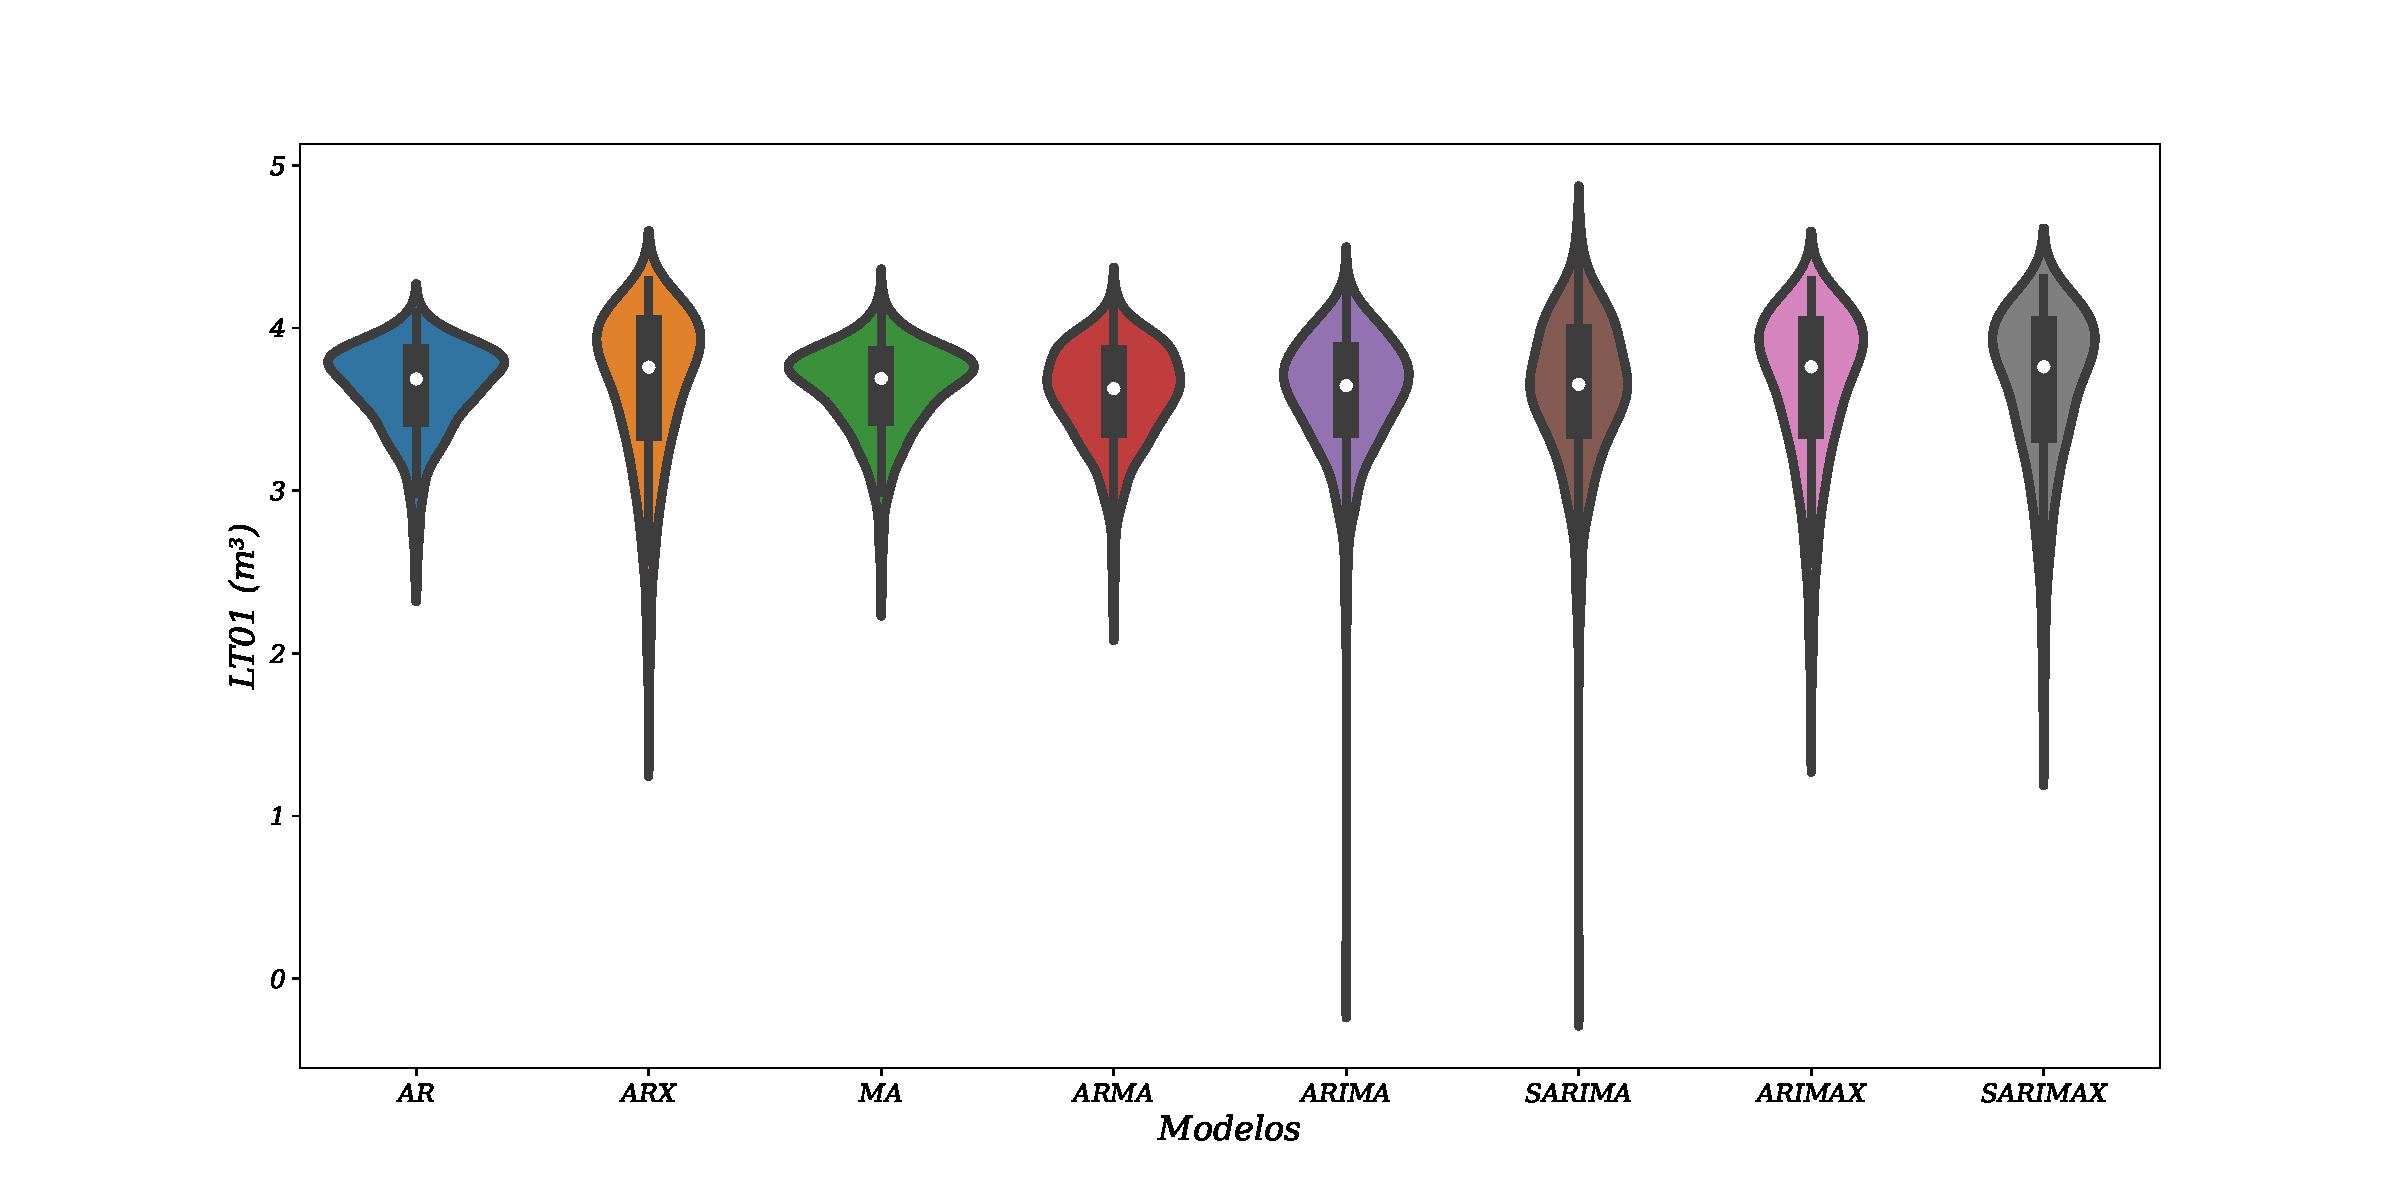
\includegraphics[width=\linewidth]{Resultados/Figuras/modelos-arima}
	
	
\end{figure}

Na Figura \ref{fig:violin-lr-xgb-lgbm-rf}, é feita uma comparação entre os modelos de gradiente e regressor. Esses modelos, por serem mais robustos e utilizar técnicas de otimização mais avançadas, mostram-se superiores aos modelos comparados. O modelo XGBoost, em particular, é identificado como superior em relação aos outros modelos na análise.

\begin{figure}[!htb]
	\centering
	\caption{Comparação de modelos de regressão}\label{fig:violin-lr-xgb-lgbm-rf}
	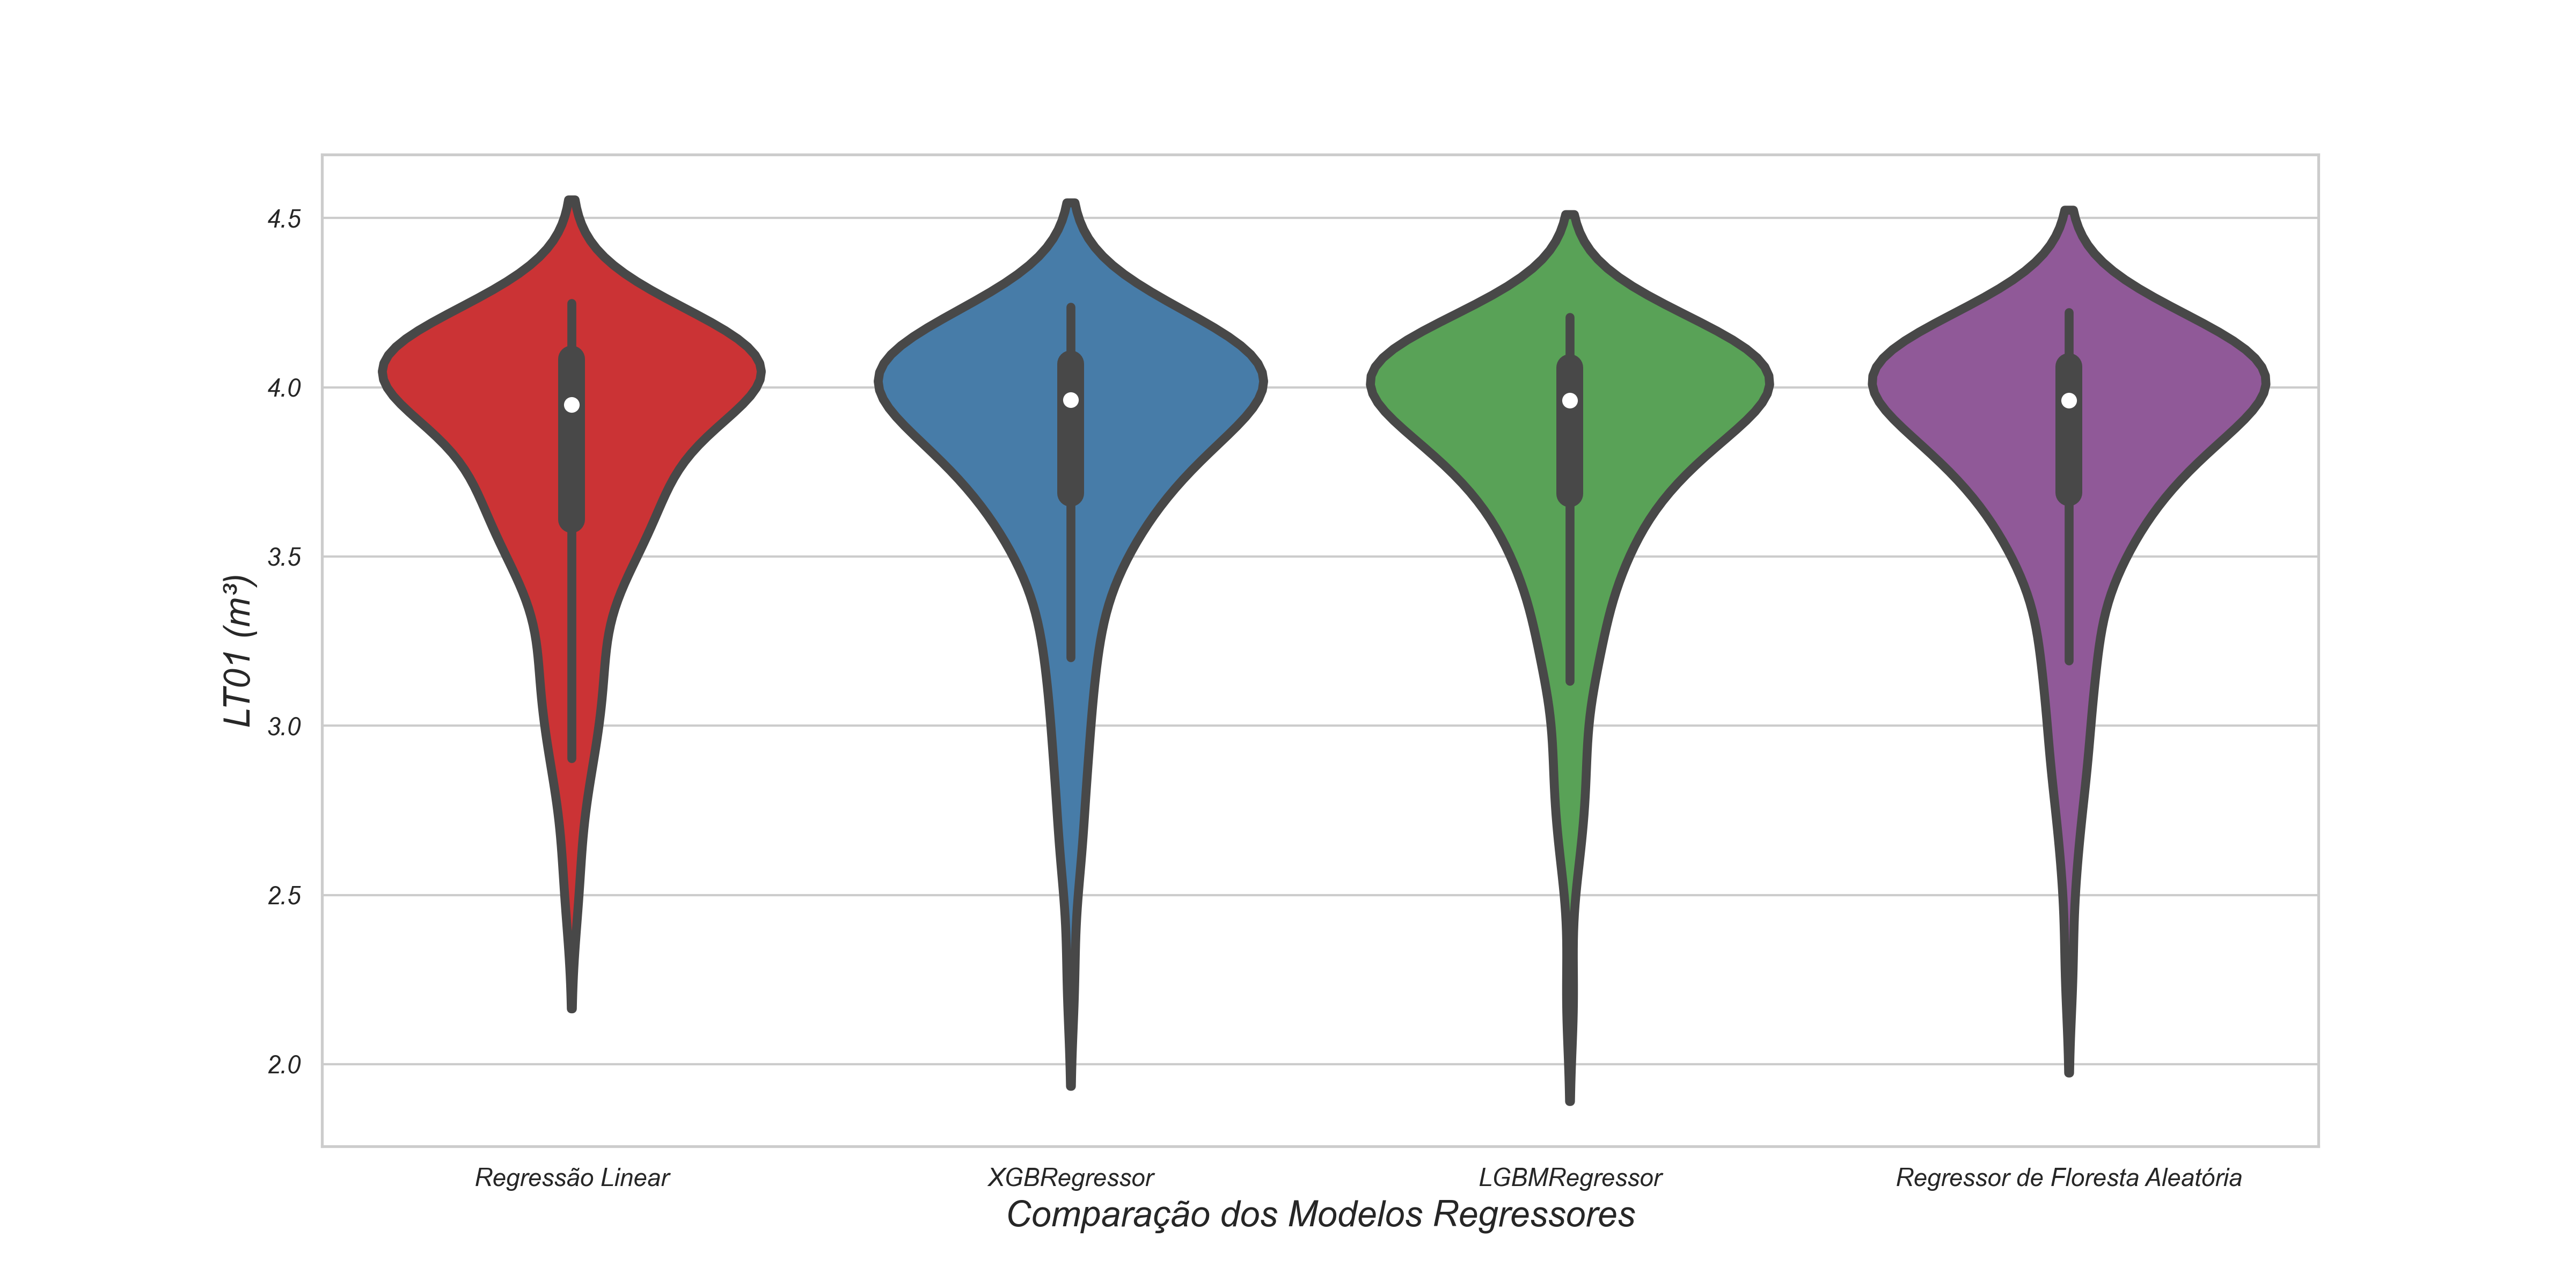
\includegraphics[width=\linewidth]{Resultados/Figuras/violin-LR-XGB-LGBM-RF}
	
\end{figure}

Na Figura \ref{fig:rrmse_comparar}, nota-se que todos os modelos trabalhados aqui, exceto o modelo LR, foram comparados em relação às métricas de desempenho. Mesmo sendo muito robustos, esses modelos não conseguiram obter um resultado tão bom quanto o RNN.
\begin{figure}[!htb]
	\centering
	\caption{Comparação dos modelos na métrica RRMSE\label{fig:rrmse_comparar}}
	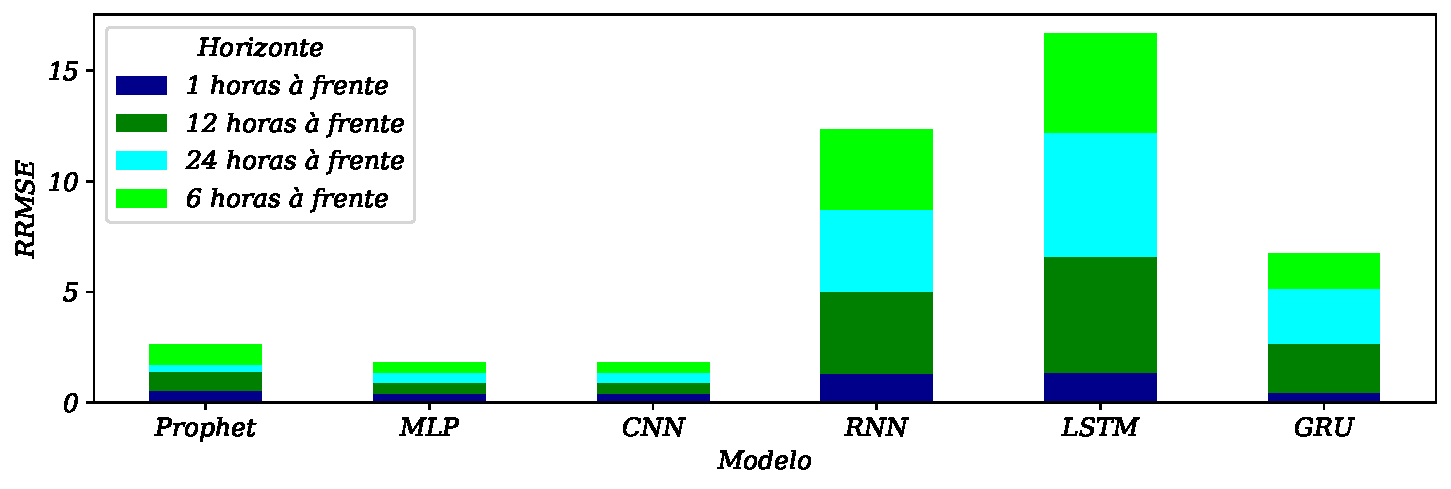
\includegraphics[width=\linewidth]{Resultados/Figuras/rrmse_comparar}
\end{figure}

\begin{figure}[!htb]
	\centering
	\caption{Comparação dos modelos nas métricas sMAPE, MAE e RRMSE\label{fig:basic_comparar}}
	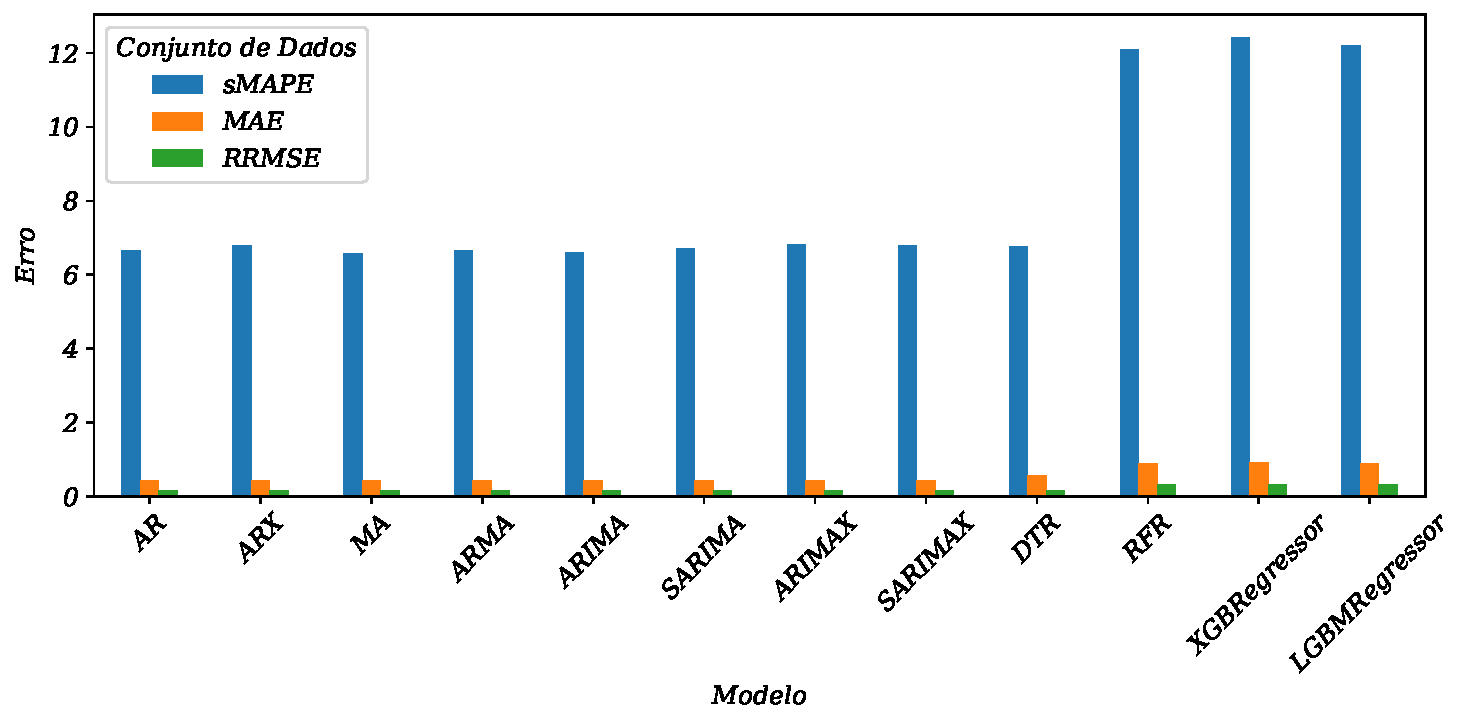
\includegraphics[width=\linewidth]{Resultados/Figuras/basic_comparar}
\end{figure}



A avaliação da eficácia dos modelos ARIMA em previsões de longo prazo emprega o teste de Ljung-Box, conforme detalhado nas Tabelas \ref{tb:lbtrn} a \ref{tb:lbcm} ilustram a acurácia dos modelos ARIMA ao longo do tempo, com valores menores sendo destacados em \textbf{negrito}  para facilitar a interpretação. Modelos como ARX, ARIMAX e SARIMAX, que incorporam variáveis exógenas, demonstram um desempenho superior nesse contexto. Esses modelos não lineares apresentam uma capacidade de previsão robusta em horizontes temporais mais longos, diferenciando-se positivamente dos outros modelos ARIMA. Na Figura \ref{fig:modelos-arima}, são selecionados os modelos ARIMA e seus antecessores. Esses modelos têm suas limitações, tanto para horizontes de previsão de curto prazo quanto para horizontes de longo prazo. Nessa comparação no gráfico de violino, são combinados vários outros gráficos em um só, como o gráfico de barras e o \textit{boxplot}. Esse gráfico pode fornecer várias informações, mas o objetivo aqui é identificar apenas o melhor modelo entre os modelos ARIMA.

Como essa série não apresentou uma estacionariedade bem definida e os dados não a tornaram estacionária, os modelos que não têm sazonalidade mostraram-se superiores, tais como AR, MA, ARX, ARMA, ARIMA e ARIMAX. O modelo ARIMAX demonstrou ser bastante robusto para este caso, mas mesmo assim, modelos mais básicos como AR e MA ainda apresentaram resultados melhores.

\begin{table}[H]
	\centering		
	\caption{Comparação dos modelos Ljung Box: Modelos ARIMA com defasagem de 10 para previsão de longo prazo na demanda de água}
	
	\begin{subtable}{0.46\linewidth}
		\centering
		\caption{\textbf{Treinamento}} \label{tb:lbtrn}
		\begin{tabular}{@{}ccc@{}}
			\toprule
			\multirow{5}{*}{\begin{tabular}[c]{@{}c@{}}Ljung \\ Box\end{tabular}} & \multirow{5}{*}{\begin{tabular}[c]{@{}c@{}}Estatística\\ de Teste\end{tabular}} & \multirow{5}{*}{\begin{tabular}[c]{@{}c@{}}Valor \\ De p\end{tabular}} \\
			& & \\
			& & \\
			& & \\
			& & \\ \midrule
			ARX & 59,677 & \textbf{0,000} \\
			AR & 52,312 & \textbf{0,265} \\
			MA & 57,268 & \textbf{0,000} \\
			ARMA & \textbf{6,945} & \textbf{0,731} \\
			ARIMA & 16,724 & 0,081 \\
			SARIMA & 48,505 & \textbf{0,000} \\
			ARIMAX & 89,931 & \textbf{0,000} \\
			SARIMAX & 29,093 & \textbf{0,000} \\ \bottomrule
		\end{tabular}
	\end{subtable}
	\hfill
	\begin{subtable}{0.46\linewidth}
		\centering
		\caption{\textbf{Teste}} \label{tb:lbtst}
		\begin{tabular}{@{}ccc@{}}
			\toprule
			\multirow{5}{*}{\begin{tabular}[c]{@{}c@{}}Ljung \\ Box\end{tabular}} & \multirow{5}{*}{\begin{tabular}[c]{@{}c@{}}Estatística\\ de Teste\end{tabular}} & \multirow{5}{*}{\begin{tabular}[c]{@{}c@{}}Valor \\ De p\end{tabular}} \\
			& & \\
			& & \\
			& & \\
			& & \\ \midrule
			ARX & 47,177 & \textbf{0,000} \\
			AR & 49,965 & 0,444 \\
			MA & 77,884 & \textbf{0,000} \\
			ARMA & \textbf{1,545} & 0,999 \\
			ARIMA & \textbf{5,354} & 0,866 \\
			SARIMA & 24,663 & \textbf{0,006} \\
			ARIMAX & 36,738 & \textbf{0,000} \\
			SARIMAX & 21,236 & \textbf{0,020} \\ \bottomrule
		\end{tabular}
	\end{subtable}
	
	\vspace{1em}
	
	\begin{subtable}{0.46\linewidth}
		\centering
		\caption{\textbf{Validação}} \label{tb:lbvld}
		\begin{tabular}{@{}ccc@{}}
			\toprule
			\multirow{5}{*}{\begin{tabular}[c]{@{}c@{}}Ljung \\ Box\end{tabular}} & \multirow{5}{*}{\begin{tabular}[c]{@{}c@{}}Estatística\\ de Teste\end{tabular}} & \multirow{5}{*}{\begin{tabular}[c]{@{}c@{}}Valor \\ De p\end{tabular}} \\
			& & \\
			& & \\
			& & \\
			& & \\ \midrule
			ARX & \textbf{5,108} & 0,884 \\
			AR & 4,360 & 0,930 \\
			MA & 46,252 & \textbf{0,000} \\
			ARMA & \textbf{7,515} & 0,676 \\
			ARIMA & \textbf{7,738} & 0,654 \\
			SARIMA & 28,998 & \textbf{0,001} \\
			ARIMAX & \textbf{6,115} & \textbf{0,000} \\
			SARIMAX & \textbf{4,443} & 0,925 \\ \bottomrule
		\end{tabular}
	\end{subtable}
	\hfill
	\begin{subtable}{0.46\linewidth}
		\centering
		\caption{\textbf{Inteiro}} \label{tb:lbcm}
		\begin{tabular}{@{}ccc@{}}
			\toprule
			\multirow{5}{*}{\begin{tabular}[c]{@{}c@{}}Ljung \\ Box\end{tabular}} & \multirow{5}{*}{\begin{tabular}[c]{@{}c@{}}Estatística\\ de Teste\end{tabular}} & \multirow{5}{*}{\begin{tabular}[c]{@{}c@{}}Valor \\ De p\end{tabular}} \\
			& & \\
			& & \\
			& & \\
			& & \\ \midrule
			ARX & 48,870 & \textbf{0,000} \\
			AR & 49,432 & \textbf{0,035} \\
			MA & 57,629 & \textbf{0,000} \\
			ARMA & \textbf{10,053} & \textbf{0,436} \\
			ARIMA & \textbf{10,053} & \textbf{0,436} \\
			SARIMA & \textbf{10,053} & \textbf{0,436} \\
			ARIMAX & 70,458 & \textbf{0,000} \\
			SARIMAX & \textbf{2,897} & \textbf{0,000} \\ \bottomrule
		\end{tabular}
	\end{subtable}
	
	
	\vspace{0.5cm}
	
\end{table}





